%% LyX 2.0.2 created this file.  For more info, see http://www.lyx.org/.
%% Do not edit unless you really know what you are doing.
\documentclass[12pt,oneside,english]{book}
\usepackage{lmodern}
\renewcommand{\sfdefault}{lmss}
\renewcommand{\ttdefault}{lmtt}
\renewcommand{\familydefault}{\sfdefault}
\usepackage[T1]{fontenc}
\usepackage[latin9]{inputenc}
\usepackage{listings}
\setcounter{secnumdepth}{3}
\setcounter{tocdepth}{1}
\usepackage{babel}
\usepackage{textcomp}
\usepackage{amsthm}
\usepackage{amsmath}
\usepackage{graphicx}
\usepackage[unicode=true]
 {hyperref}

\makeatletter
%%%%%%%%%%%%%%%%%%%%%%%%%%%%%% Textclass specific LaTeX commands.
\numberwithin{equation}{section}
\numberwithin{figure}{section}

\makeatother

\begin{document}

\title{SQL-Ledger User Guide}


\author{Written by\\
Sebastian Weitmann\\
Armaghan Saqib\\
\\
\\
\\
\\
\\
International SQL-Ledger Network Association}

\maketitle
\tableofcontents{}


\chapter*{Preface}

TODO


\chapter{Introduction}


\section{Introducing SQL-Ledger}

SQL-Ledger is an open source accounting/ERP solution written by Dieter
Simader. Its version 1.0 was released in Jan. 29, 1999. So as of this
writing in 2013, it is 14 years old software which is under constant
development and enhancement during this period. This makes it suitable
enough for small as well as for large businesses.

SQL-Ledger has an impressive feature set which even many commercial
/ properietary ERP solutions don't provide. Its internal design and
user interface are simple which make it easy to learn.

SQL-Ledger is a free (as in liberty) software solution which means that it comes with full source code which you can modify as you wish, redistribute it and run it for any purpose. Even reselling SQL-Ledger is allowed. 
Furthermore you don't need to worry about discovering undocumented bugs which might cost you thousands of Dollars to fix them. Another point is that the sources of the code will always be freely available which is a benefit should your
ERP-provider go out of business.

Ledger123 is an enhanced version of SQL-Ledger. It was created to
fix some of the bugs in SQL-Ledger which were not getting fixed. We
still call Ledger123 as 'Enhanced SQL-Ledger'.


\subsection{Versions}

The current release of stock SQL-Ledger is 3.0.8. Ledger123 is based
upon 3.0.3 with its enhancements. We call it Ledger123 release 3.
Ledger123 tries to incorporate all the goodness which comes from stock
SQL-Ledger. So you get best of both worlds.

To make things simple, we assume that you are using Ledger123 release
3 (Enhanced SQL-Ledger release 3). Though most of the sections would
apply equally well to the stock SQL-Ledger 3 as well as older versions.
This is particularly true if you are not using inventory related functions
because most of the enhancements in Ledger 123 are related to inventory.

Website and other resources on the Internet




\section{Getting up and running}


\subsection{Installing enhanced sql-ledger using 'git clone'}

The recommended way to download and install our enhanced SQL-Ledger
is to use 'git' package. To install git on Ubuntu, you run 'sudo apt-get
install git-core'. Once git is successfully installed, you can proceed as follows:
\begin{enumerate}
\item Download the sql-ledger github repository. You will get a fully working
sql-ledger installation which includes our enhancements. (The default
'master' branch)\\
\begin{lstlisting}
git clone git://github.com/ledger123/ledger123.git 
\end{lstlisting}

\item From now onwards you can upgrade to our latest enhancements (which
includes any latest releases from sql-ledger.com) with the following
simple commmand:\\
\begin{lstlisting}
git pull
\end{lstlisting}

\item Let us say you are not interested in our enhancements and just want
to maintain and upgrade to the sql-ledger release from sql-ledger.com.
Switch to the sql-ledger branch first time:\\
\begin{lstlisting}
git checkout -b sql-ledger origin/sql-ledger
\end{lstlisting}

\item From now onwards upgrading to official sql-ledger from sql-ledger.com
is as easy as:\\
\begin{lstlisting}
git pull
\end{lstlisting}

\item Note that you can always switch back and forth between our enhanced
sql-ledger and the official one by git checkout as:\\
\begin{lstlisting}
git checkout master # enhanced sql-ledger
git checkout sql-ledger # official sql-ledger
\end{lstlisting}

\item You can switch back to any past sql-ledger version. First see a log
of all commits and 40 chars hashes:\\
\begin{lstlisting}
git log --pretty=oneline
\end{lstlisting}

\item To revert to sql-ledger 2.8.17\\
\begin{lstlisting}
git checkout 7b15e9b
\end{lstlisting}

\end{enumerate}
SQL-Ledger Virtual Machine


\section{Our enhancements to standard SQL-Ledger}


\subsection{Departments}
\begin{enumerate}
\item Restrict user to a particular department using admin.pl. 
\item Default department for user. 
\item Department is mandatory on invoices/orders/quotes if there is at least
one department defined. 
\end{enumerate}

\subsection{Warehouses}
\begin{enumerate}
\item Warehouse transfers module.
\item Restrict user to a particular warehouse using admin.pl.
\item Default warehouse for user.
\item Track warehouse inventory from sales and purchase invoices.
\item Track inventory-in-transit between warehouse movement.
\item Warehouse is mandatory on invoices if there is at least one warehouse
defined. 
\item Warehouse onhand and activity reports. 
\end{enumerate}

\subsection{COGS}
\begin{enumerate}
\item Re-posting script which corrects cogs errors due to invoice editing. 
\item Invoice and invoice-item cogs/revenue information with gross profit
\%age. 
\item Onhand value report which shows the inventory onhand quantities and
value based upon fifo costing. 
\end{enumerate}

\subsection{Reports}
\begin{enumerate}
\item Per-invoice and per-item cogs/revenue information. 
\item Enhanced tax reports. Audit trail report. 
\item Drill-down to transactions from income statement. 
\item Invoice date and customer/vendor filter in \textquoteleft{}All Items\textquoteright{}
report. 
\item Account description in \textquoteleft{}GL Reports\textquoteright{}. 
\item Account activity report using \textquoteleft{}GL Reports\textquoteright{}. 
\item Save report search conditions and layout in user menu. Recall with
a single click. 
\end{enumerate}

\subsection{Others}
\begin{enumerate}
\item 'Add Customer', 'Add Vendor' links on invoices/orders/quotes/POS screens.
These links appear only if allowed by access control settings. 
\item Enhanced assemblies. You can get a report of all stock-assembly actions.
Warehouses are correctly updated with any assemblies made and components
used. 
\item Enhanced bank reconciliation. 
\item Added back the 'Shipping\textendash{}Transfer' function from sql-ledger
2.6. 
\item LedgerDoctor script which identifies potential problems with data
entry. 
\item CSV data import. (invoices,transactions,gl,orders,customers,vendors,parts,chart) 
\item Disabled incorrect item weight update from orders and invoices 
\item Parts group is mandatory if there is at least on group defined. 
\end{enumerate}

\section{Explanation of bugs and gotchas in official version}


\subsection{Orders}
\begin{enumerate}
\item Warehouse information is not updated when you receive orders by editing
Rcvd quantity on orders. 
\item When you make changes to invoice created from an order (add/remove
item, quantities), inventory onhand count goes out of order. This
is caused any invoice created from order does not update the inventory
onhand. 
\end{enumerate}
We have fixed these issues by not allowing to receive orders by editing
them. We also do not allow editing invoices created from orders to
avoid corrupting onhand quantities.


\subsection{COGS}
\begin{enumerate}
\item Incorrect accounting transaction is posted for sale returns. COGS
gets corrupted when you edit an invoice. 
\item We have modified the posting of sale returns to post correct cogs. 
\end{enumerate}
We have added a reposting script to correct any corrupted cogs values
when you edit an invoice.


\subsection{Warehouses}

Default warehouse functionality is broken in many ways. If somebody
is successfully using it without ledger123 enhancements, I would love
to know how?


\chapter{Setting up your business on SQL-Ledger}

The next step after successful SQL-Ledger installation is to setup
your initial business data. You need do do this before you start making
your day to day transactions.


\section{Creating your first dataset}

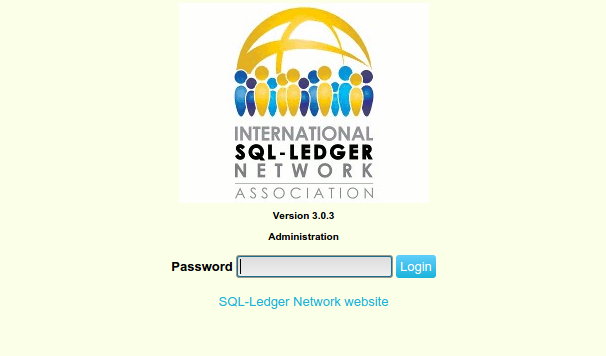
\includegraphics{admin1}

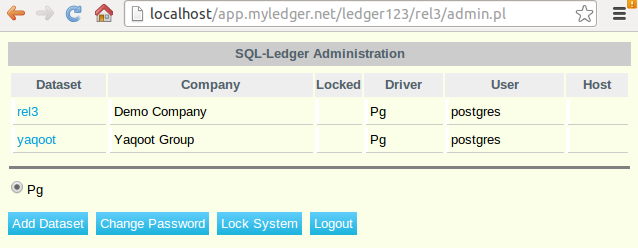
\includegraphics{admin2}

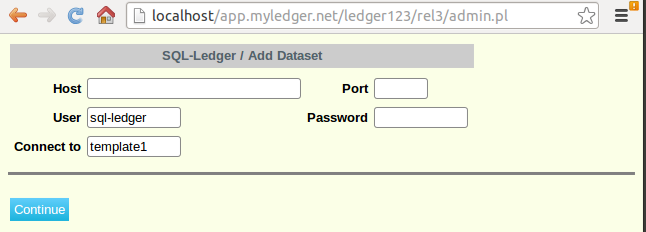
\includegraphics{admin3}

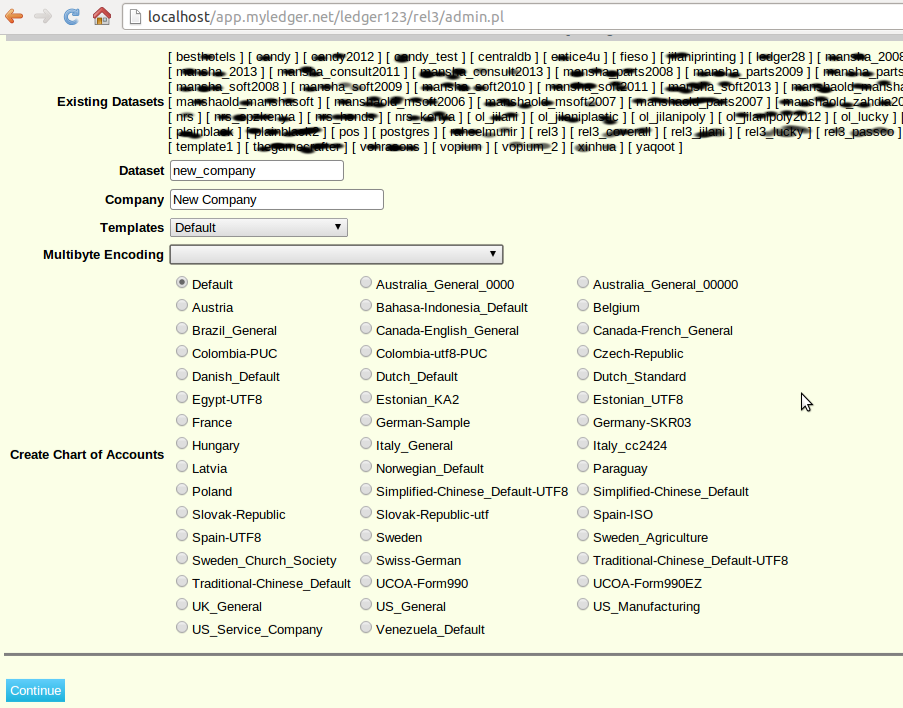
\includegraphics{admin4}

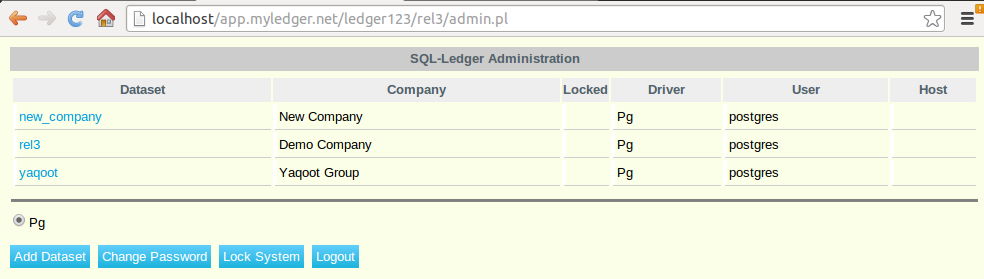
\includegraphics{admin5}


\section{Creating users and roles}


\subsection{Roles}

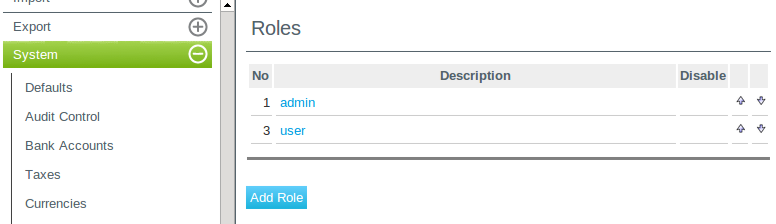
\includegraphics{role1}

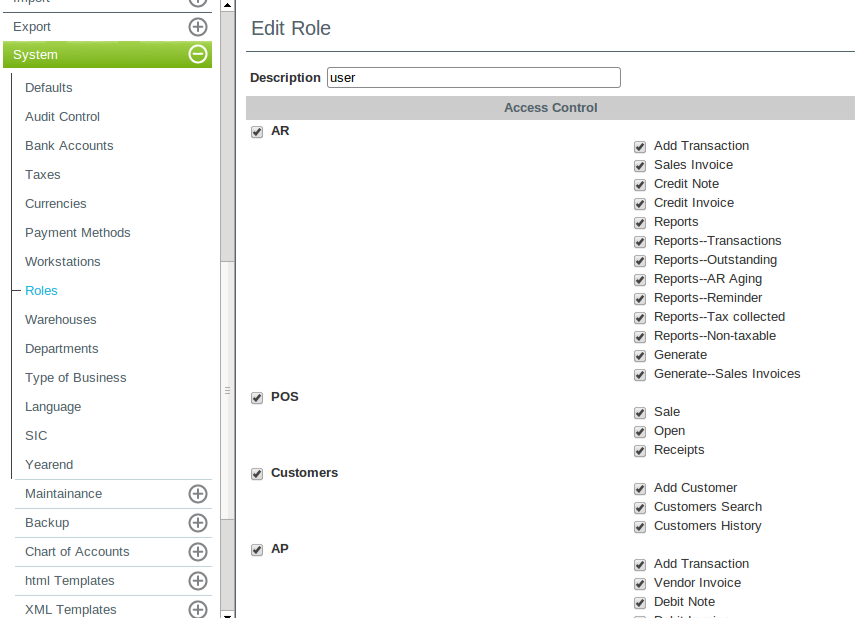
\includegraphics{role2}


\subsection{Users}

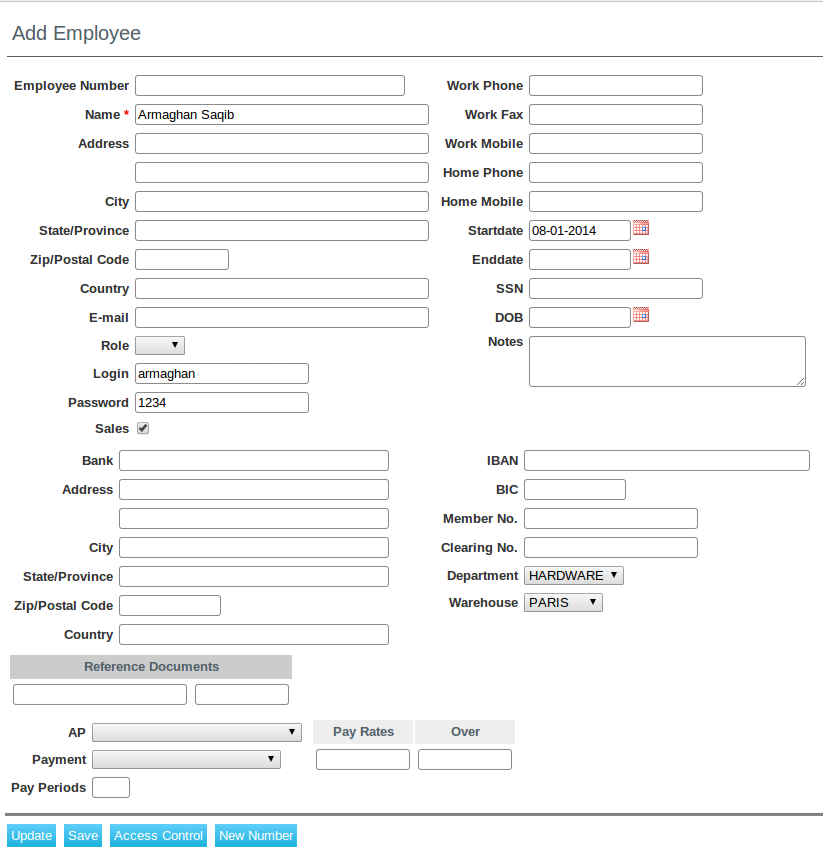
\includegraphics{user1}

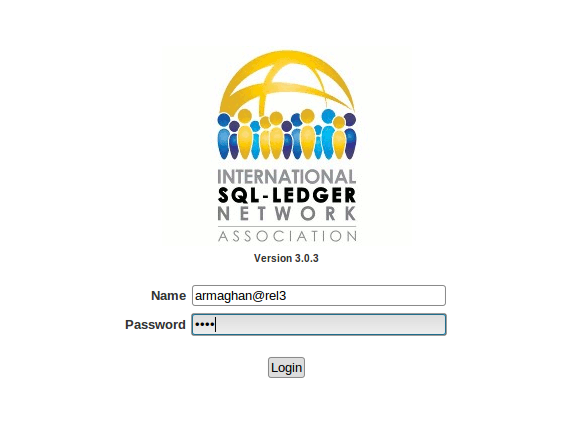
\includegraphics{user3}

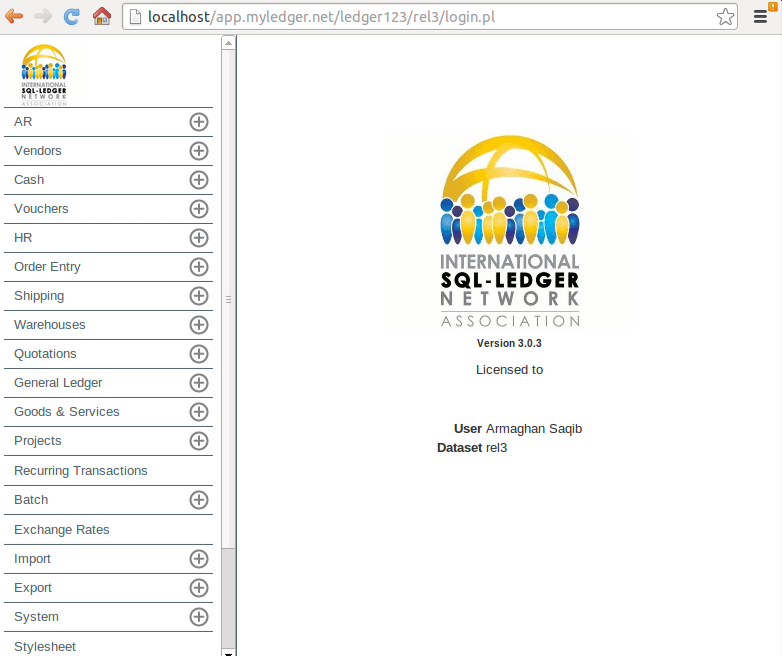
\includegraphics{user4}


\section{Defaults}

System\textendash{}Defaults menu allows you to setup your company,
address and related information in SQL-Ledger. Document numbering
is also controlled by system defaults.

We setup defaults for document numbers as shown on the following screen
shot. You can change these to your liking or organizational needs.

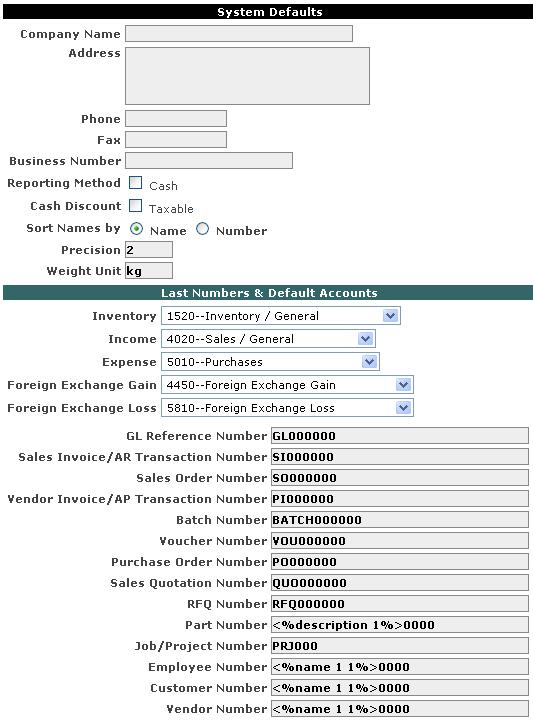
\includegraphics[scale=0.5]{defaults}


\section{Customers}

You need to add at least one customer before creating invoices. Use
Customers--Add Customer to add new customers.

To change existing customers, first you list them using Customers\textendash{}Reports\textendash{}Search.
Customers are listed with hyperlinks to edit each customer.

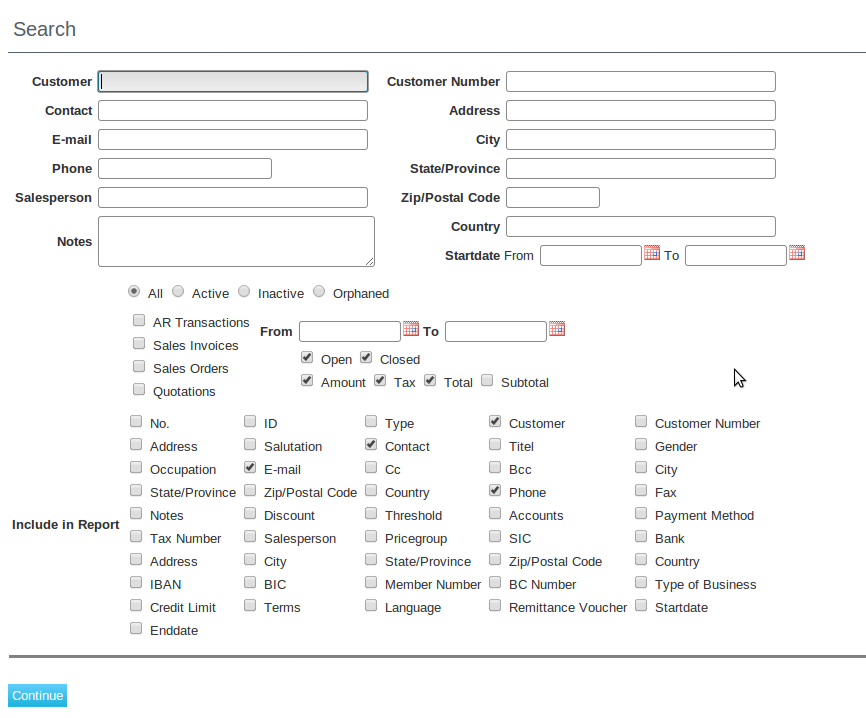
\includegraphics[scale=0.5]{customer-search1}

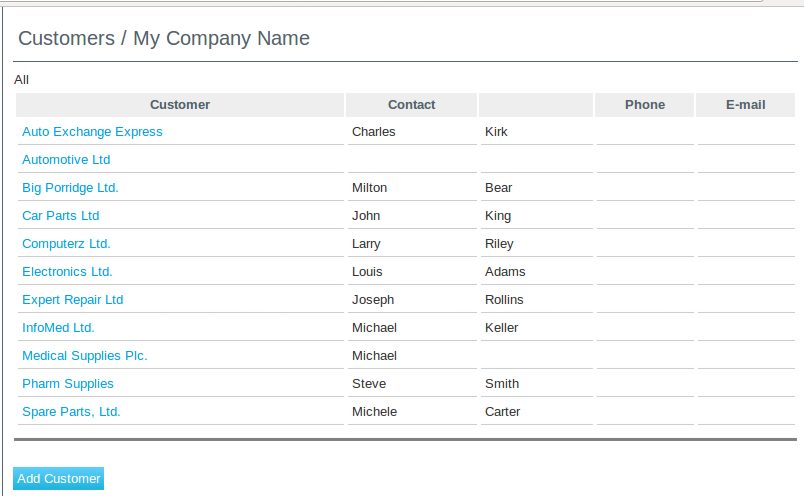
\includegraphics{customer-search2}

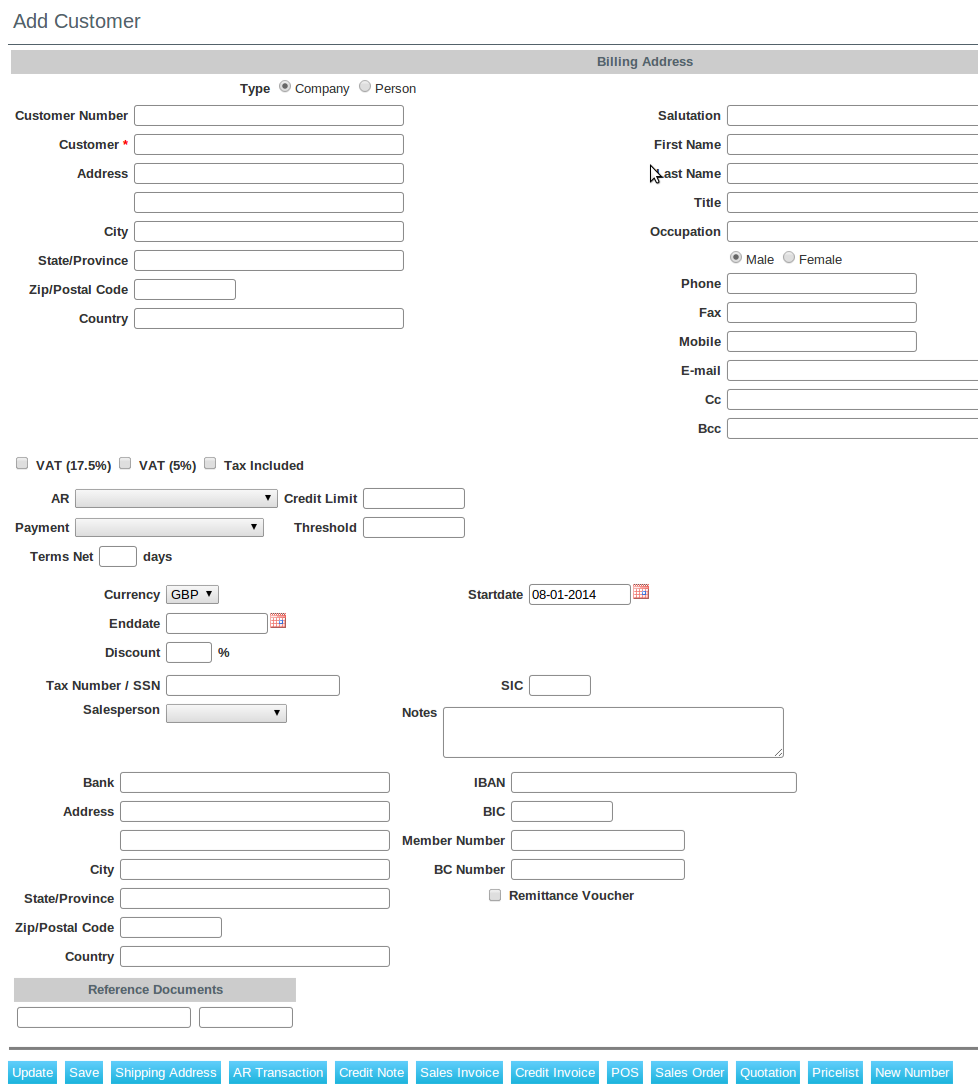
\includegraphics{customer1}


\section{Vendors}

You need to add at least one vendor before creating invoices. Use
Vendors\textendash{}Add Vendor to add new vendors.

To change existing vendors, first you list them using Vendors\textendash{}Reports\textendash{}Search.
Vendors are listed with hyperlinks to edit each vendor.

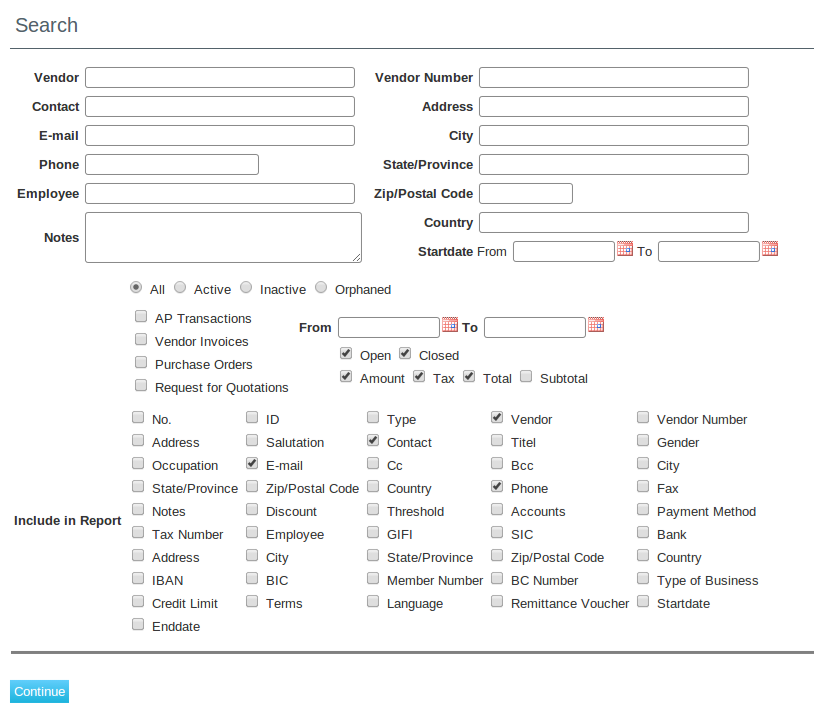
\includegraphics[scale=0.5]{vendor-search1}

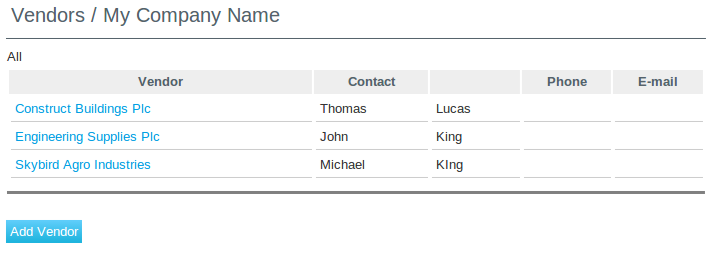
\includegraphics{vendor-search2}

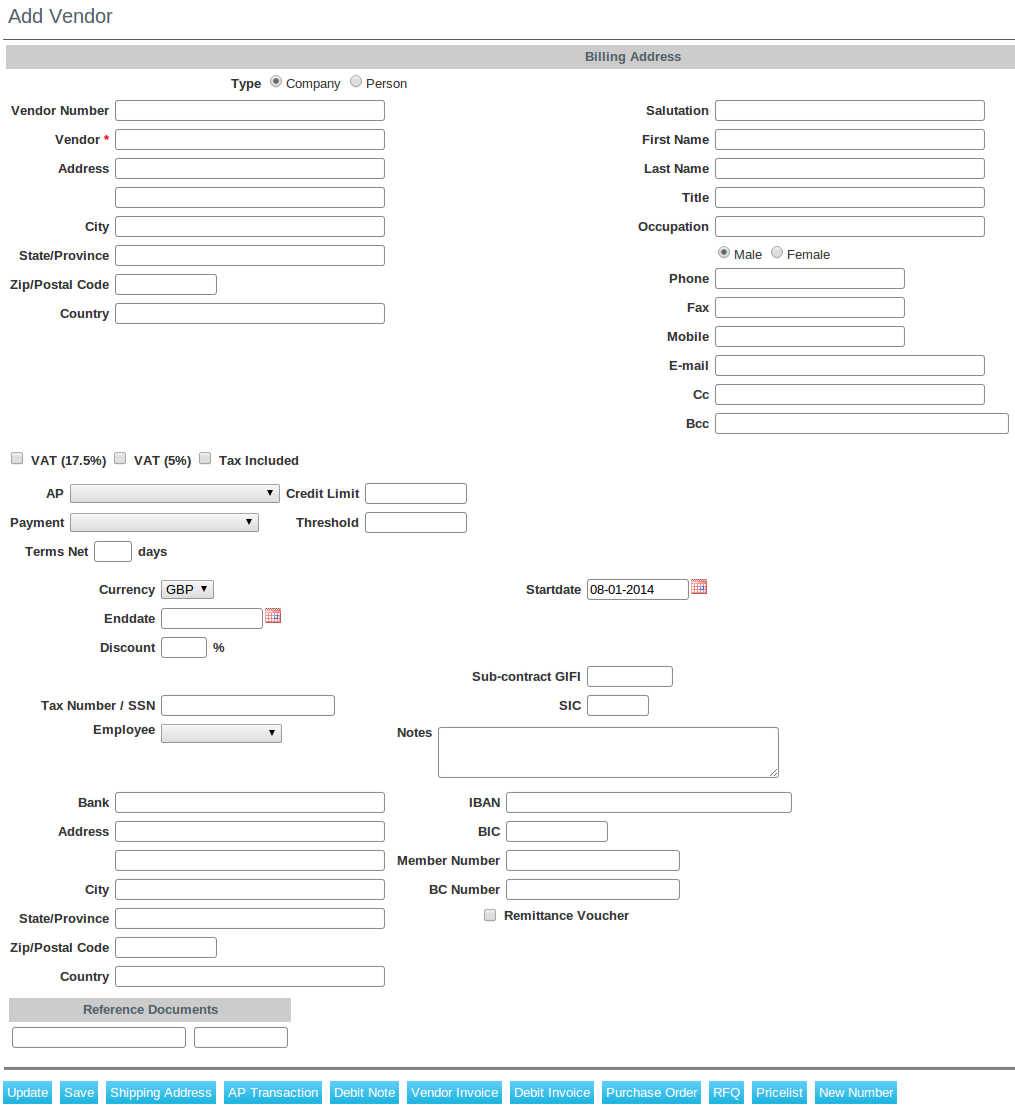
\includegraphics{vendor1}


\section{Type of Business }


\section{Employees }


\section{Departments}

Departments are optional and can be used to classify transactions
according to a department code.


\subsection{Managing Departments}

Departments can be added, changed or deleted using 'System\textendash{}Departments'
menu option.

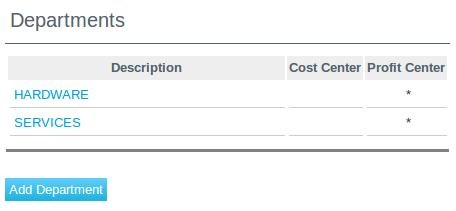
\includegraphics[scale=0.5]{department1}

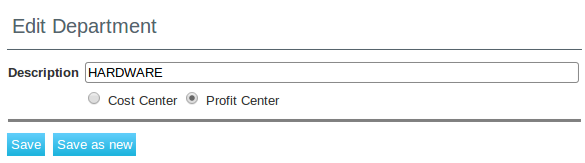
\includegraphics{department2}

SQL-Ledger departments can be mapped to the various departments (sales,
purchase etc.), branches (London, Oxford etc.) or product divisions
(Product 1, Product2 etc.) within your organization.

Departments can be marked as 'Cost Center' or 'Profit Center'. Cost
center departments appear only in purchasing module. Profit center
departments appear both in purchasing and sales modules.

You can also change 'Department' to anything you like (eg.Branch)
using the sql-ledger language customization feature. Note: Departments
lookup does not appear on transaction forms unless you define at least
one department from System\textrightarrow{}Departments menu option.


\subsection{Default Department}

You can define a default default for users through sql-ledger administrative
interface. You can also restrict the user to view and make transactions
to his department only by setting his role to User. Users with role
Administrator, Manager, Supervisor always have access to all departments.

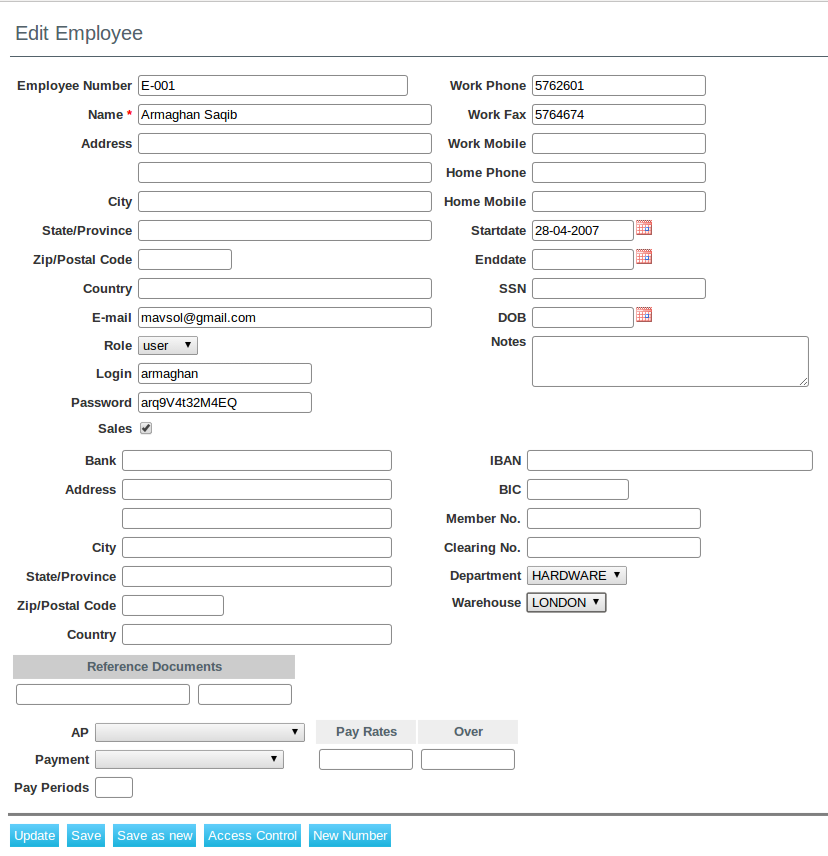
\includegraphics[scale=0.5]{department3}


\subsection{Using Departments}

Once departments are defined you can specify them in your invoices,
orders, quotations and other transactions.

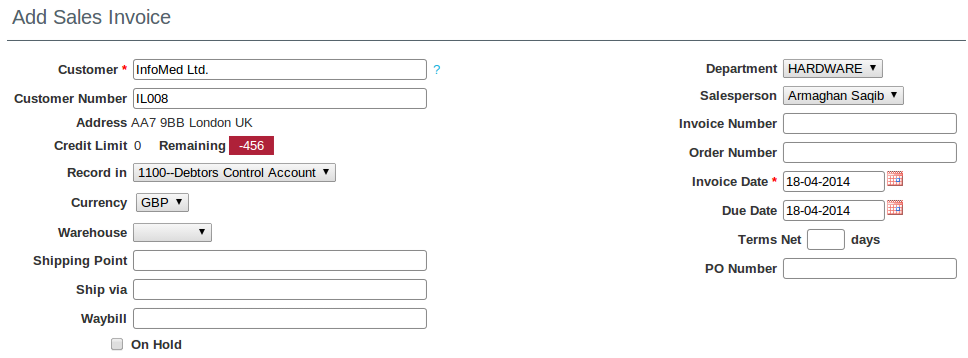
\includegraphics{department4}


\subsection{Reports}

Reports allow you to view all or department specific transactions.

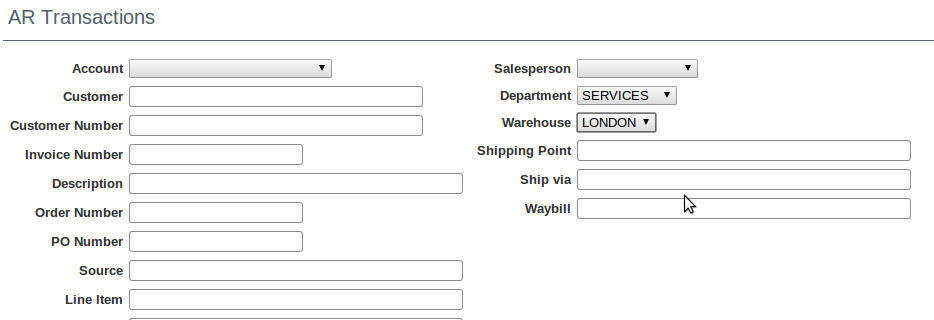
\includegraphics{department5}

Income Statement and Balance sheet can also be compared and displayed
by department.

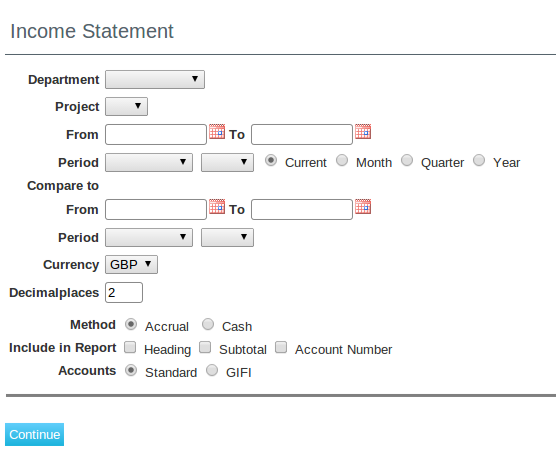
\includegraphics{department6}

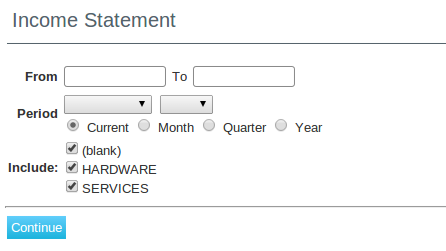
\includegraphics{department7}

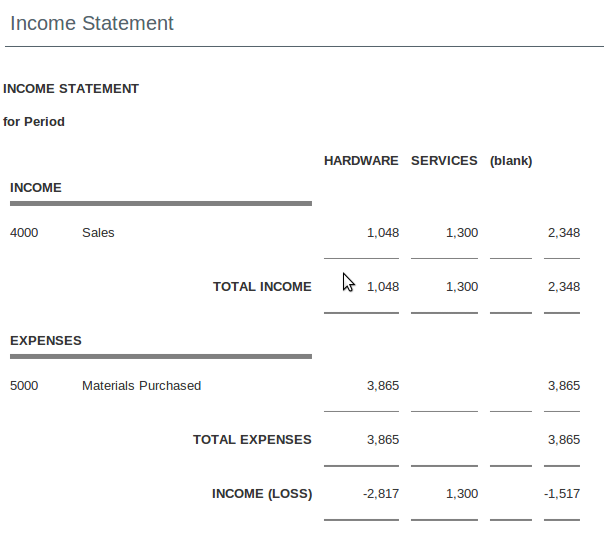
\includegraphics{department8}


\section{Projects}

Projects are optional and can be used for following things:
\begin{enumerate}
\item Track income and expenses to specific projects using invoices and
general ledger transactions. 
\item Enter time card data. 
\end{enumerate}
Notes Projects lookup appears on transactions forms only if you have
created at least one project.


\subsection{Managing Projects}

You can add or change projects through Projects menu.

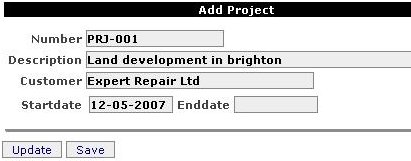
\includegraphics{project1}


\subsection{Using Projects}

Once you have defined projects, you can use them in sales and purchase
invoices.

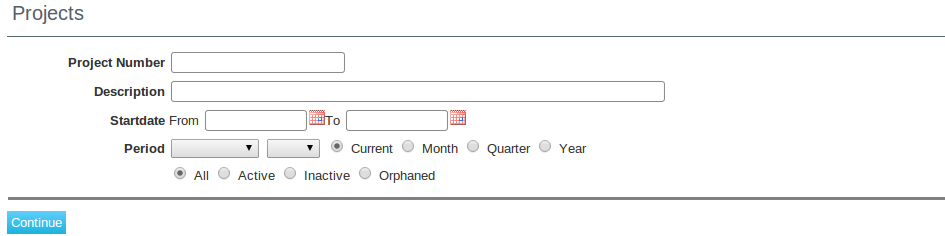
\includegraphics{project2}


\section{Chart of Accounts}


\section{Templates}

Print forms for invoices, orders, quotations and financial reports
can be customized by you by editing form templates. There are three
type of templates:


\subsection{HTML Templates}

HTML templates are easier to modify because it of widespread knowledge
of html. Only basic html knowledge is required to edit html templates.

TODO: Attach:templates1.jpg


\subsection{Latex Templates}

Latex templates are bit complex to understand and modify but offer
complete control over printed invoice, order or quotation forms. See
below for basic introduction to latex.

TODO: Attach:templates3.jpg


\subsection{Text Templates. Used only with Point-of-Sale interface}

Text templates are used only for Point-of-Sale receipts printing.
These templates allow you to print on 40 character receipt printers.

TODO: Attach:templates4.jpg


\subsection{Editing Templates}

Templates can be edit through sql-ledger. When you click on a template,
it is displayed with 'Edit' button at the end of the template. Clicking
the 'Edit' button will open the template in a text box where it can
be edited and saved.

Attach:templates2.jpg


\subsection{Template Variables}

Sql-ledger replaces actual data into templates using variables which
we call template variables. Template variables are enclosed within
<\% and \%>.

Here are some template variables to give you an idea. The best way
to view all these template variables and understand their usage is
by going through existing templates.

\begin{lstlisting}[basicstyle={\footnotesize\ttfamily}]
<%name%>
<%address1%>
<%address2%>
<%city%>
<%state%>
<%zipcode%>
<%country%>
<%contact%>
<%invnumber%>
<%invdate%>
<%duedate%>
<%ordnumber%>
<%employee%>
<%shippingpoint%>
<%shipvia%>
<%runningnumber%>
<%number%>
<%description%>
<%deliverydate%>
<%qty%>
<%unit%>
<%sellprice%>
<%discountrate%>
<%linetotal%>
\end{lstlisting}



\subsection{Template control commands}

Template processing engine in sql-ledger allows simple if statement
and loops. Example of these are described below:


\subsubsection{'if' is used to print a column data conditionally}

\begin{lstlisting}[basicstyle={\footnotesize\ttfamily}]
<%if contact%>
  <br><%contact%>
  <br>
<%end contact%>

<%if taxincluded%>
   <th colspan=7 align=right>Total</th>
   <td colspan=2 align=right><%invtotal%></td>
<%end taxincluded%>

<%if not taxincluded%>
   <th colspan=7 align=right>Subtotal</th>
   <td colspan=2 align=right><%subtotal%></td>
<%end taxincluded%>

<%if paid%>
   <tr>
      <th colspan=7 align=right>Paid</th>
      <td colspan=2 align=right>- <%paid%></td>
   </tr>
<%end paid%>
\end{lstlisting}



\subsubsection{'for' loop to print all lines on an invoice}

\begin{lstlisting}[basicstyle={\footnotesize\ttfamily}]
<%foreach number%>
        <tr valign=top>
          <td align=right><%runningnumber%>.</td>
          <td><%number%></td>
          <td><%description%></td>
          <td><%deliverydate%></td>
          <td align=right><%qty%></td>
          <td><%unit%></td>
          <td align=right><%sellprice%></td>
          <td align=right><%discountrate%></td>
          <td align=right><%linetotal%></td>
        </tr>
<%end number%>

<%foreach tax%>
  <tr>
     <th colspan=7 align=right><%taxdescription%> on <%taxbase%> @ <%taxrate%> %</th>
     <td colspan=2 align=right><%tax%></td>
  </tr>
<%end tax%>
\end{lstlisting}



\subsection{An Introduction to Latex}

Latex is a complete collection of software tools to create high quaility
print documents. Latex templates are used in SQL-Ledger to create
high quality print forms like invoices, purhcase orders etc.

Latex is included with Redhat distributions (rpm -qa | grep tetex). 

For FreeBSD, you can install the teTex port from /usr/ports/print/te\TeX{}.

Latex migh seem overwhelming to a new comer but it is really a simple
toolkit to use for customizing the SQL-Ledger templates. In this very
short introduction of Latex, we shall go through the basic document
format and its use in SQL-Ledger.

Here is 'Hello world!' in latex.


\subsubsection{Create a text file (hello.tex) in your home folder with following
text:}

\begin{lstlisting}[basicstyle={\footnotesize\ttfamily}]
\documentclass[a4paper,11pt]{article}
\begin{document}
Hello world!
\end{document}
\end{lstlisting}



\subsubsection{Compile this tex file into dvi file and use xdvi to view it:}

\begin{lstlisting}[basicstyle={\footnotesize\ttfamily}]
latex hello.tex
xdvi hello.dvi
\end{lstlisting}



\subsubsection{You can also convert it to pdf:}

\begin{lstlisting}[basicstyle={\footnotesize\ttfamily}]
pdflatex hello.tex
xpdf hello.pdf
\end{lstlisting}



\subsection{Structure of a Latex Document}

Latex commands start with a backslash (\textbackslash{}). Parameters
can follow the command. Optional parameters are enclosed in {[}{]}
while mandatory ones are enclosed in \{\}. \{\} can also be used to
terminated a command mixed within some text (to make it easier to
understand the command for the compiler). Special characters in latex
(\#, \$, \%, \textasciicircum{}, \&, \_, \{, \}, \textasciitilde{})
are escaped with \textbackslash{} except for the \textbackslash{}
character itself (because is used to break a line). To use literal
backslash (\textbackslash{}) use can use special command \$\textbackslash{}backslash\$.

Single line comments start with \% while multi-line comments can be
enclosed between \textbackslash{}begin\{comment\} and \textbackslash{}end\{comment\}
structure.

Every latex document starts with \textbackslash{}documentclass with
parameters ({[}a4paper,11pt{]}\{article\}) following it.


\section{Parts}

Parts are tangible items you keep in your stock. You purchase them
from your vendors and sell them to your customers for profit.

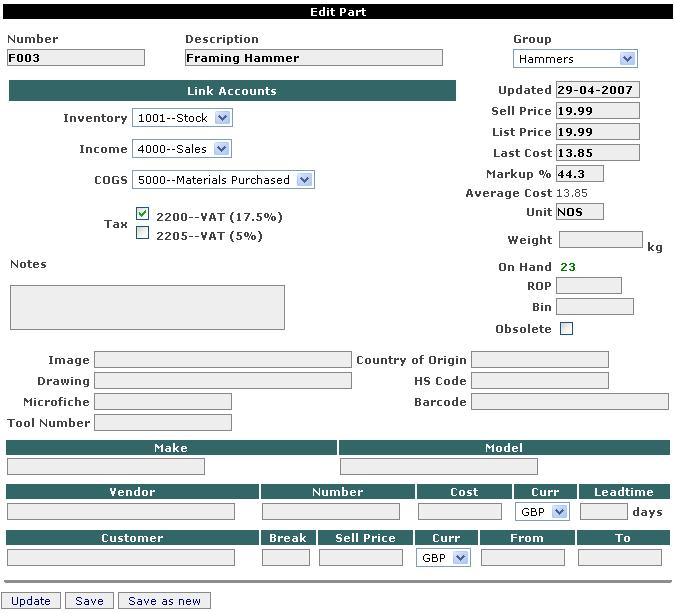
\includegraphics[scale=0.5]{parts1}


\section{Services}

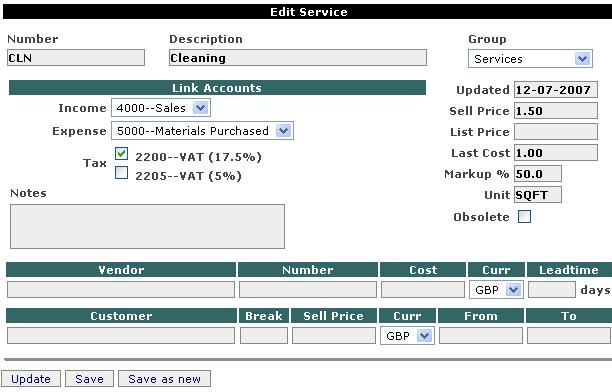
\includegraphics[scale=0.5]{services1}


\section{Assemblies}

An assembly is composed of components which are individual parts in
the inventory or other sub-assemblies. Assemblies in SQL-Ledger allow
you to do manage your manufacturing process.

Work flow for using assemblies:
\begin{enumerate}
\item Define assemblies. Goods \& Services--Add Assembly.
\item Build assemblies. Goods \& Services--Stock Assembly. Individual parts
are removed and assemblies are added to the stock inventory.
\item Sell assembly items like any other item.
\end{enumerate}
Please note that you cannot buy parts defined as assemblies.


\subsection{Define assemblies}

As assembly is just like any other inventory item in your sql-ledger
with the additional information about its components. You define new
assemblies using Goods and Service -- Add Assembly.

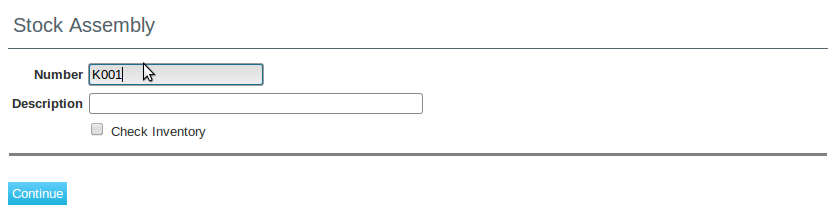
\includegraphics[scale=0.5]{assembly1}


\subsection{Stock assemblies}

This option reduces the quantities of the components and increases
the onhand quantity of the assemblies. COGS is not recorded at this
point.

COGS for the assembly is recorded from individual components when
you sell the assembly. FIFO allocation also occurs at the time of
sale. (Rows are inserted in invoice table for component parts with
assemblyitem=TRUE)

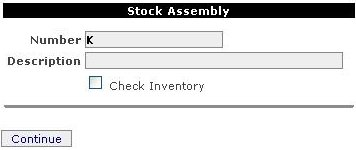
\includegraphics[scale=0.5]{stock1}


\subsection{Reports}

More Reports--Goods and Services--Stock Assembly gives you a list
of your Stock Assembly actions. This report lists the parts taken
out of assembly as well as assemblies built.

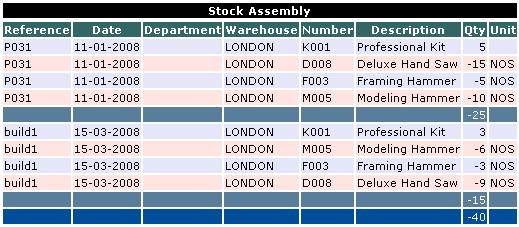
\includegraphics[scale=0.5]{stock5}

Goods and Services--Assemblies gives you list of all or selected assemblies
with their components.

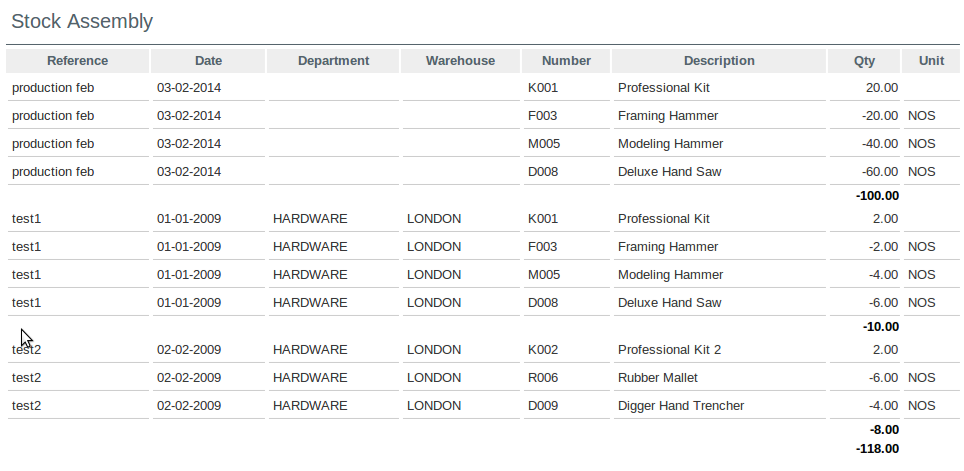
\includegraphics[scale=0.5]{stock3}

Goods and Servers--Components gives you a list order by partnumber
and the assembly in which it is used.

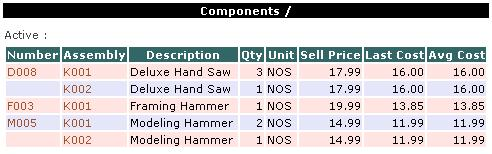
\includegraphics[scale=0.5]{stock4}

Work Order You can print work order for a sales orders. Work order
lists all component parts required to fullfil a given order of assembly
items.

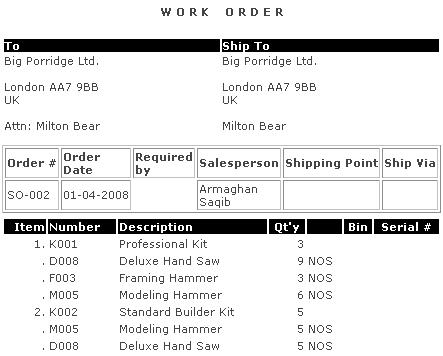
\includegraphics[scale=0.5]{workorder1}


\section{Labour/Overhead}

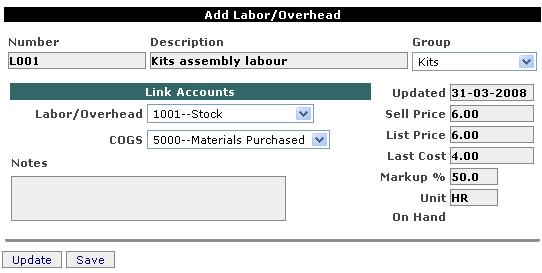
\includegraphics[scale=0.5]{labour1}


\section{Groups}

Groups are used to group togather the parts and services. You can
filter parts and services reports by selecting a group on search screens.

Groups have another useful functionality. When you check the POS button
box during group add or change, they appear as buttons on POS (point-of-sale)
screens making it easier to select items within each group.

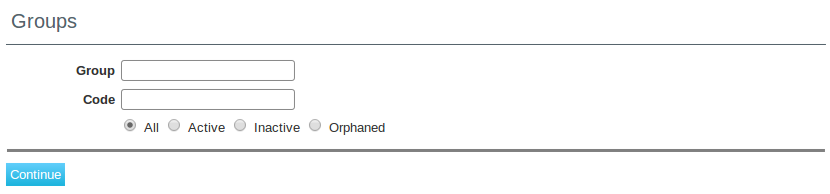
\includegraphics{group1}


\section{Pricegroups}

SQL-Ledger has very flexiable pricing mechanism. For example:
\begin{enumerate}
\item You can define customer specific prices for each part. 
\item You can define quantity breaks. (If someone buys 10 units instead
of 1, he/she can automatically gets lower price.) 
\item And you can specify start and end dates to offer a special price during,
for example, Christmas season. 
\end{enumerate}
Price groups take this concept further and allow you to define 'groups'
of special prices. Let us say you sell to distributor, dealer and
end-user. Each of these groups of customers gets tiered discount/price.

There are three steps to use price groups:
\begin{enumerate}
\item Create three price groups; distributor, dealer and enduser. (Goods
\& Services-Add Pricegroup)
\item Define item prices for these price groups. To do this, open the item
for editing and select the price group and set the price according
to the price group tier. Leave the customer column blank. Repeat this
for all items. (Clicking 'Update' will allow you to set prices for
multiple pricegroups for a single item.) 
\item Open the customer record for editing and set the applicable price
group for that customer.
\end{enumerate}
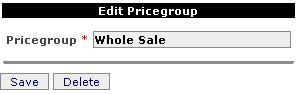
\includegraphics{pricegroup1}


\section{Warehouses}

Warehouses are optional and can be used to manage your inventory at
more than one physical place.

Important: Once you have defined warehouses, these are no longer optional
and you cannot save a transaction (invoice or transfer) without specifying
a warehouse.

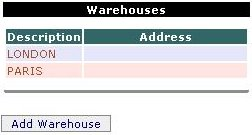
\includegraphics{warehouse1}


\subsection{Adding warehouses}

You can add, change or delete warehouses through 'System\textendash{}Warehouses'
option.

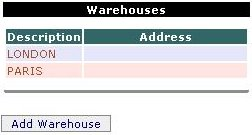
\includegraphics{warehouse1}


\subsection{Default warehouse}

You can define a default warehouse for users through administrative
interface. You can restrict a user to view and make transactions to
his warehouse by setting his role to User. Users with role Administrator,
Manager, Supervisor always have access to all warehouses.

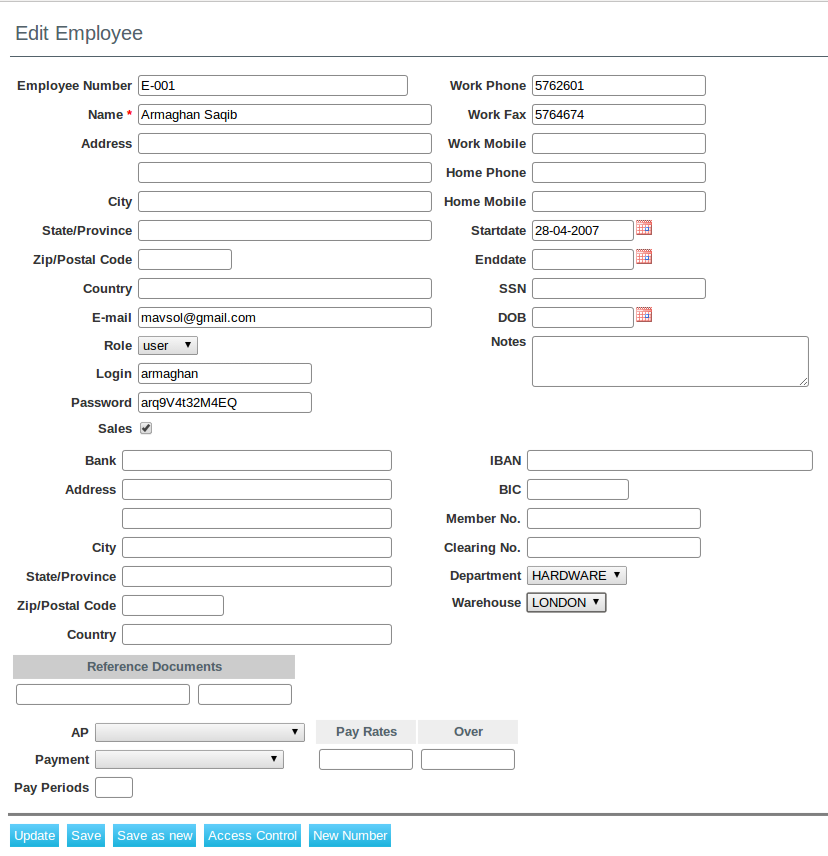
\includegraphics{department3}


\subsection{Using warehouses}

Warehouse drop down is enabled on relevant transactions forms once
you define at least one warehouse. When you purchase goods, quantity
is added to the specified warehouse. When you sell goods, quantity
is subtracted from the specified warehouse.

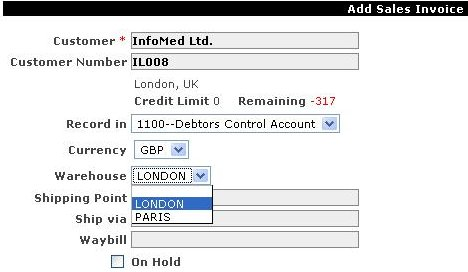
\includegraphics{warehouse2}


\subsection{Warehouse transfers}

You can move inventory between warehouses by using 'Warehouses\textendash{}Add
Transfer' menu option.

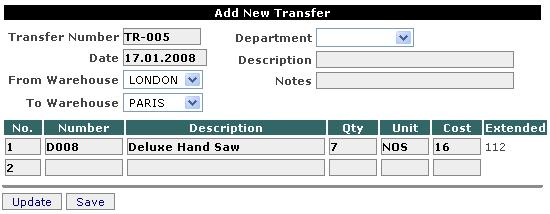
\includegraphics{warehouse4}


\subsection{Transfers delivered}

Some companies also need to track the in-transit goods between warehouse
transfers. Delivered date is usually different from transfer date.

When you login, you will see the number of transfers which have been
sent to your default warehouse but not received by you yet.

To 'receive' the transfers, click the 'Warehouses\textendash{}Reports\textendash{}Deliveries'
menu option, specify criteria and click Continue to display the transfers
pending to be received. Here you specify the dates when the goods
were delivered at 'your' warehouse and click 'Save Delivered'.

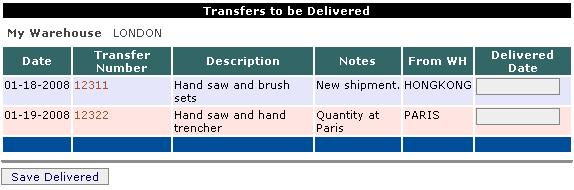
\includegraphics{warehouse_pending2}


\subsection{Reports}
\begin{enumerate}
\item Goods \& Services\textendash{}Parts report provides summary of your
on hand quantity at selected or all warehouses. Click 'Warehouse'
check box to display onhand by warehouse.
\item Warehouses\textendash{}Reports\textendash{}Transfers gives you a list
of transfers. Summary lists transfer transactions and Detail lists
all items in each transfer transaction. You can click on transfer
number hyper link to edit the transfer.
\item Warehouses\textendash{}Reports\textendash{}Onhand gives you inventory
onhand for all warehouses or for a particular warehouse. 
\item Warehouses\textendash{}Reports\textendash{}Activity gives you all
activity of a particular item or all items. Select warehouse to see
the activity in a particular warehouse. Activity report shows activity
from purchase invoices, sales invoices and transfers.
\end{enumerate}
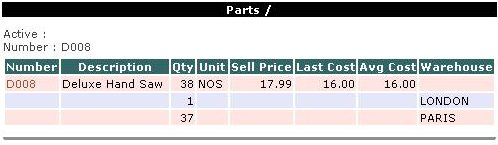
\includegraphics{warehouse3}


\subsection{Enabling multiple warehouses for old dataset}

If you have upgraded your sql-ledger installation with our enhanced
version, you need to run few queries to bring your old data in sync
with the new warehouses structure.

Assemblies are a special case. In standard sql-ledger, 'Stock Assembly'
action does not create any transaction/log and directly updates the
onhand quantities in parts table. If you are using assemblies, you
will almost always need to adjust the components and assemblies quantities
after running these queries. See step 4 below.

Important: Make sure you have a current backup before doing this.

TODO: Copy queries and other text here. See how code can be formatted
properly


\section{Translations}


\section{Taxes}

Defining and using taxes in sql-ledger is a four step process:


\subsection{Define tax accounts in chart}

You create (or edit) tax accounts in chart of accounts using System\textendash{}Accounts
menu option.

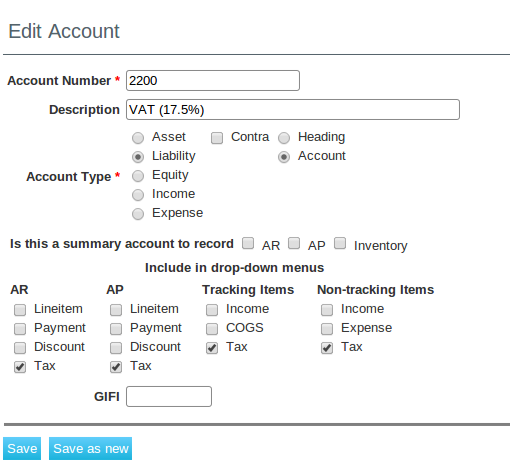
\includegraphics[scale=0.5]{tax0}

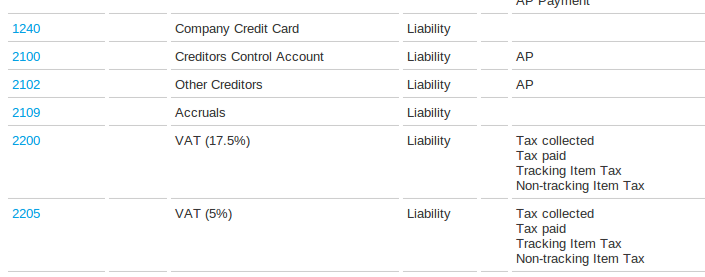
\includegraphics{tax2}


\subsection{Define tax percentages}

You set percentages for each tax using System\textendash{}Taxes menu
option.

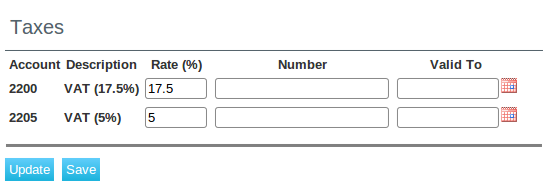
\includegraphics[scale=0.5]{tax1}


\subsection{Mark Items/services as taxable}

You mark each part or service taxable during add or edit process.
You do this using Goods \& Services menu option.

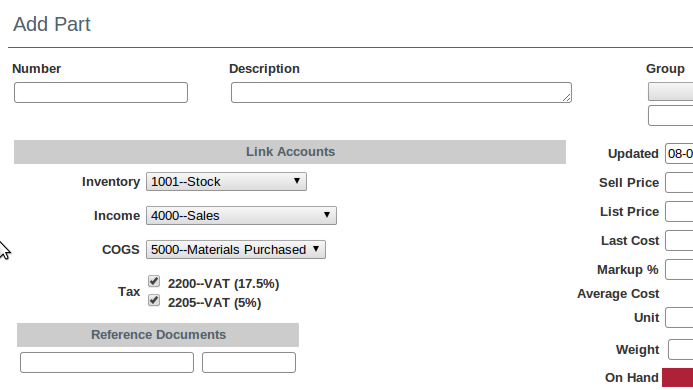
\includegraphics[scale=0.5]{tax4}


\subsection{Mark customers/vendors for applicable taxes}

Tax will not be calculated for your customers or vendors unless you
mark them as taxable.

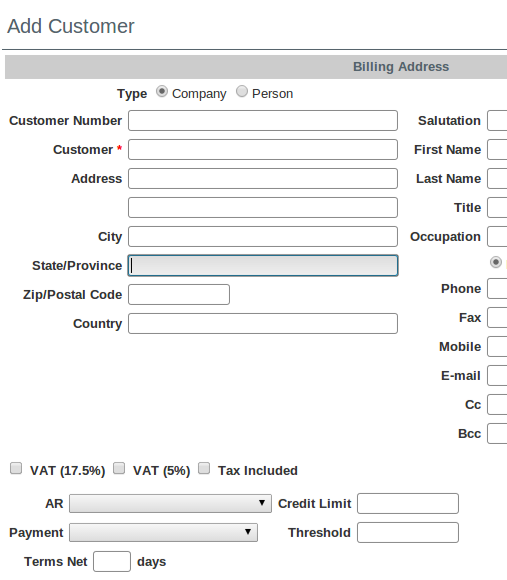
\includegraphics[scale=0.5]{tax3}


\section{Data import from other applications}

Sometimes you need to import your sales data into sql-ledger which
was produced elsewhere.

You might have a web store where you download your daily sales in
CSV format and want to import it into Sql-Ledger. Or you are just
moving to sql-ledger from your legacy accounting software and want
to move all existing data from old software to sql-ledger.

Following sections provide detailed steps for importing CSV text files.


\subsection{Sale invoices}

Sales invoices can be imported from text files.


\subsubsection{Format your data}

Here is a sample import data. You prepare data in this format and
save it in a text file. The last column AR is accounts receivable
account number which is 1100 in UK chart of accounts.

If your data contains invoices with more than one item, repeat the
row with same invoice header information and change the item number
and price information. SQL-Ledger will import all these rows as a
single invoice. (See invoice number A100 above)

For list of additional data columns that can be imported see step
4.

\begin{lstlisting}[basicstyle={\scriptsize\ttfamily},breaklines=true]
invnumber,transdate,duedate,customernumber,curr,invoicedescription,partnumber,
qty,sellprice,employeenumber,AR,department,warehouse 
A100,10/12/2008,10/30/2008,AE001,GBP,Invoice description comes here,B001,10,102,E-001,1100,HARDWARE,LONDON
A100,10/12/2008,10/30/2008,AE001,GBP,Invoice description comes here,F003,6,69,E-001,1100,HARDWARE,LONDON
A101,10/12/2008,10/31/2008,CP002,GBP,Test description,F003,2,32,E-002,1100,SERVICES,PARIS
A102,10/13/2008,11/1/2008,ER003,GBP,Sale of goods,T007,6,12,E-003,1100,SERVICES,LONDON
A103,10/14/2008,11/2/2008,SP007,GBP,Sale,K001,12,32,E-004,1100,HARDWARE,PARIS
\end{lstlisting}



\subsubsection{Upload and preview}

Using Import--Sales Invoices menu option, upload this file into Sql-Ledger.
You will be shown what will be imported before actual import is done.
At this point you can check and uncheck the invoices to be imported.

\includegraphics[scale=0.5]{import_invoices}


\subsubsection{Confirm data import}

When you click the Import Sales Invoices button, invoices will be
imported. You will be show which invoices were imported successfully.

\includegraphics[scale=0.5]{import_invoices2}


\subsubsection{Additional data which can be imported}

Sample csv file provided above contains only the most commonly used
columns. Here is the complete list.

transdate

invnumber

customernumber

curr

duedate

employeenumber

ordnumber

quonumber

datepaid

shippingpoint

shipvia

waybill

terms

notes

intnotes

language\_code

ponumber

cashdiscount

discountterms

partnumber

description

sellprice

discount

qty

unit

serialnumber

projectnumber

deliverydate

AR

taxincluded


\subsection{Receipts and Payments}

You can import payments and match them to invoices using 'Import\textendash{}Payments'.
Following points should be kept in mind.
\begin{enumerate}
\item Payments are matched first on Invoice DCN column and then, if no match
is found, on payment amount. 
\item Both AR and AP invoices are matched with payments. 
\item The amount matched is calculated as debit minus credit.
\end{enumerate}

\subsubsection{Format your data}

Create or format the data in a CSV file with structure similar to
the given below.

\begin{lstlisting}[basicstyle={\scriptsize\ttfamily}]
datepaid,memo,debit,credit,dcn
2008/11/03,"payment ref 2121",,38.76,
2008/10/04,"cash payment",,527.5, 2008/10/10,"CC Receipt",,243.08,
2009/11/01,"Payment matched by DCN",,1401.72,1122
\end{lstlisting}



\subsubsection{Upload and perview}

Import script will read the CSV file and match the payments to AR
or AP invoices first on DCN Number and then on invoice due amount,
if needed.

In this example, one AP invoice is matched on amount and the other
one is matched on DCN number. The other two are AR invoices which
are matched on amount.

\includegraphics[scale=0.5]{import_payments2}


\subsubsection{Confirm data import}

Once you click 'Import Payments', payments are imported and applied
to the matched invoices.

\includegraphics[scale=0.5]{import_payments3}


\subsubsection{Advanced receipts/payments import}
\begin{enumerate}
\item You can easily change the script to match the payments on other invoice
columns like invoice number. The procedures to modify are 'sub payments'
in 'SL/IM.pm' and 'sub im\_payment' in 'bin/mozilla/im.pl'.
\item To match payments only to AR (or AP) invoices, change the UNION queries
in SL/IM.pm to select invoices from AR or AP only as required.
\end{enumerate}

\subsection{AR/AP Transactions}

You can import AR and AP transactions.

For AR transactions, format your data using following sample:

\begin{lstlisting}[basicstyle={\scriptsize\ttfamily}]
invnumber,customernumber,transdate,amount,description,notes,source,memo
00003,AE001,10-11-07,2030,"desc1","notes1","source1","memo1"
00004,CP002,07-12-07,3213,"desc1","notes2","source2","memo2"
00005,SP007,09-12-07,-200,"desc1","notes3","source3","memo3"
\end{lstlisting}


For AP transactions, format your data using following sample:

\begin{lstlisting}[basicstyle={\scriptsize\ttfamily}]
invnumber,vendornumber,transdate,amount,description,notes,source,memo 
00003,CB001,10-10-08,2030,"desc1","notes1","source1","memo1" 
00004,ES002,10-12-08,3213,"desc2","notes2","source2","memo2" 
00005,SA003,12-12-08,-200,"desc3","notes3","source3","memo3"
\end{lstlisting}



\subsection{General Ledger}

This feature will help you to move your data from most of the accounting
software to sql-ledger in few easy steps:


\subsubsection{Format your data}

Format your data according to following sample. Keep in mind that:
\begin{enumerate}
\item Import script creates one GL transaction for each unique 'reference'
number. 
\item There can be any number of lines (rows) in each transaction. 
\item Account must exist in chart of accounts Debits and credits must be
equal before the CSV file can be imported.
\end{enumerate}
\begin{lstlisting}[basicstyle={\scriptsize\ttfamily},breaklines=true]
reference,transdate,description,notes,accno,debit,credit,source,memo
GL001,01-20-2008,"Paid for training,support",Next session in 2009,8203,124,0,23211,new hiring
GL001,01-20-2008,"Paid for training,support",Next session in 2009,1230,0,124,23211,new hiring
GL002,10-19-2008,"Overdue pymt for inv 11,12,13",,1230,204,0,"11,12,13", 
GL002,10-19-2008,"Overdue pymt for inv 11,12,13",,1102,0,204,"11,12,13",
GL003,11-20-2008,Invalid transaction for testing,This account is not in chart,00121,0,255,source2,memo2
\end{lstlisting}



\subsubsection{Upload and preview}

Using 'Imports\textendash{}GL Transaction' load the CSV file into
sql-ledger. Import script will show the rows which contain valid account
number and can be imported.

\includegraphics[scale=0.5]{gl_import2}


\subsubsection{Confirm data import}

Click Import GL to finish the import script. Transactions successfully
imported will be show on the next page.

\includegraphics[scale=0.5]{gl_import3}


\subsection{Customers and Vendors}

Customer and Vendor import is similar (except the number column which
is customernumber or vendornumber).

Prepare your data file using the sample text provided below. (Change
customernumber to vendornumber for vendor import)

\begin{lstlisting}[basicstyle={\scriptsize\ttfamily},breaklines=true]
customernumber,name,firstname,lastname,contacttitle,phone,fax,email,notes,address1,address2,city,state,zipcode,country
001,Ledger123,Armaghan,Saqib,Consultant,,,saqib@ledger123.com,"These are, just, sample notes",,,London,,"AA7 8BB",UK
\end{lstlisting}



\subsection{Parts}


\subsubsection{Format your data}

Format your data according to following sample format. Please note
that:
\begin{enumerate}
\item Import procedure assigns a unique parts\_id to each part imported
or group created.
\item Duplicates are not allowed and duplicate check is done on partnumber.
\end{enumerate}
\begin{lstlisting}[basicstyle={\scriptsize\ttfamily},breaklines=true]
partnumber,description,unit,partsgroup,listprice,sellprice,lastcost,rop,bin,image,drawing,notes
B002,"Brush Set",NOS,brush,9.99,9.99,7,150,TOP,noimage,brush.jpg,notes about brush set 
D010,"Deluxe Hand Saw",NOS,SAW,17.99,17.99,16,50,TOP,saw.jpg,nodrawing,notes about hand saw 
D011,"Digger Hand Trencher",NOS,Picks & Hatchets,18.99,18.99,15,200,TOP,,nodrawing,notes about hand saw
\end{lstlisting}



\subsubsection{Upload and preview}

To start the import process, click 'Data Import\textendash{}Parts'
in the menu. Following page will be displayed. Click 'Browse' to select
your CSV file, mark the taxes applicable and select the account links
(Defaults are enough most of the time) Click 'Continue' when done.
You will be presented with the following screen. On this screen you
can mark the parts to be imported by checking or un-checking the checkbox
on each line.

Please note:
\begin{enumerate}
\item The parts which are already in the system (based on partnumber) will
not imported. (You will not see a check box with them)
\item Parts groups which are new will be added. These are marked by a '+'
sign after group name.
\end{enumerate}
\includegraphics[scale=0.5]{import_parts1}

\includegraphics[scale=0.5]{import_parts2}


\subsubsection{Confirm data import}

Click 'Import Parts'. Your CSV file will be processed and parts will
be imported. Any new groups will also be added. You will see an output
like the following:

\includegraphics[scale=0.5]{import_parts3}


\subsection{Vendor price list}


\subsubsection{Format your data}

\begin{lstlisting}[basicstyle={\scriptsize\ttfamily},breaklines=true]
partnumber,vendornumber,vendorpartnumber,lastcost,curr,leadtime
B001,CB001,V-CB001,10,GBP,15 B002,ES002,,14,GBP,45 M004,SA003,,21,GBP,30
\end{lstlisting}



\subsubsection{Upload and preview}

Click 'Data Import\textendash{}Parts Vendors', specify the file with
the 'Browse' button and click 'Import Parts Vendors' button. Following
page will be displayed. Here you can un-check the rows which you do
not want to import. Rows with invalid vendor number or partnumber
will not have the checkbox.

\includegraphics[scale=0.5]{import_partsvendors}


\subsection{Customer price list}


\subsubsection{Format your data}

\begin{lstlisting}[basicstyle={\scriptsize\ttfamily}]
partnumber,customernumber,pricegroup,pricebreak,sellprice,validfrom,validto,curr
B001,AE001,PG1,10,11,03-01-2008,,GBP
B002,BP011,,20,12,,03-01-2009,GBP
M004,CP002,,15,20,03-01-2008,03-05-2008,GBP
D08,CP002,test,25,25,,,GBP
\end{lstlisting}



\subsubsection{Upload and preview}

Click 'Data Import\textendash{}Parts Customers', specify the file
with the 'Browse' button and click 'Import Parts Customers' button.
Following page will be displayed. Here you can un-check the rows which
you do not want to import. Rows with invalid customer number or partnumber
will not have the checkbox.

\includegraphics[scale=0.5]{import_partscustomers}


\subsection{Chart of accounts}


\subsubsection{Format your data}
\begin{enumerate}
\item Prepare your chart of accounts in your spreadsheet software according
to the sample given below. 
\item Upload the chart csv file using 'Import\textendash{}Chart' menu option. 
\item Check/uncheck the accounts to be imported and click continue to import
the selected accounts.
\end{enumerate}
\begin{lstlisting}[basicstyle={\scriptsize\ttfamily},breaklines=true]
accno,description,charttype,category,link 
1000,"CURRENT ASSETS",H,A, 
1060,"Checking Account",A,A,AR_paid:AP_paid 
1065,"Petty Cash",A,A,AR_paid:AP_paid 
1200,"Accounts Receivables",A,A,AR 
1205,"Allowance for doubtful accounts",A,A, 
1500,"INVENTORY ASSETS",H,A, 
1520,"Inventory / General",A,A,IC 
1530,"Inventory / Aftermarket Parts",A,A,IC 
1800,"CAPITAL ASSETS",H,A,
\end{lstlisting}



\chapter{Running your business on SQL-Ledger }


\section{AR}


\subsection{AR Transaction}

AR--Add Transaction menu option is used to create AR Transactions.
These transactions allow you to record your sales in correct GL accounts
without creating an invoice.

\includegraphics[scale=0.4]{ar1}


\subsection{Sales Invoice}

Sales invoices are created using AR--Sales Invoice menu option. The
only mandatory columns are Customer and Invoice Date. Rest of the
columns can be left blank.

Once you enter an item (part, service) and click 'Update', a new line
opens. This way you can enter any number of items (parts, services
etc.) in the detail portion of the invoice.

\includegraphics[scale=0.35]{ar2}

\includegraphics{ar3}


\subsection{Transactions Report}

\includegraphics{artrans}

\includegraphics{artrans2}

\includegraphics{artrans3}


\subsection{Aging Report}

\includegraphics{ar-aging-search}

\includegraphics{ar-aging-summ}

\includegraphics{ar-aging-detail}


\subsection{Reminders}

\includegraphics{reminder1}

\includegraphics{reminder2}


\subsection{Customer History Reports}

\includegraphics{customer-history1}

\includegraphics{customer-history2}

\includegraphics{customer-history3}


\section{Receipts}

You can record cash receipts from customer while creating invoices
(for cash sales) or afterward using Cash--Receipt menu.

\includegraphics[scale=0.5]{receipt}


\section{AP}


\subsection{AP Transactions}

\includegraphics{ap1}


\subsection{Purchase Invoice}

\includegraphics{ap2}

\includegraphics{ap3}


\subsection{Transactions Report}

\includegraphics{aptrans}

\includegraphics{aptrans2}


\subsection{Aging Report}

\includegraphics{ar-aging-search}

\includegraphics{ap-aging2}

\includegraphics{ap-aging3}


\subsection{Vendor History}

\includegraphics{vendor-history1}

\includegraphics{vendor-history2}

\includegraphics{vendor-history3}


\section{Payments}


\section{General Ledger}


\subsection{Add Transaction}

\includegraphics{gl1}


\subsection{Reports}

\includegraphics{gl2}

\includegraphics{gl3}

\includegraphics{gl4}


\section{Recurring Transactions}

Recurring Transactions allow you to auto-generate pre-defined invoices,
transactions and orders.

This feature can be used for the following:
\begin{enumerate}
\item Recurring billing to a customer (For rent, web hosting, school fee,
installment etc.) 
\item Recurring billing from your vendor 
\item Monthly orders to your vendors or from your customers. 
\item Monthly payroll posting using GL Recurring Transactions. 
\item Month-end adjustments and allocations.
\end{enumerate}

\subsection{Scheduling}

To generate the next number for a given transaction, leave the Next
Number blank.

\includegraphics[scale=0.5]{recurring2}


\subsection{Generating}

When recurring transactions are due you are reminded when you login
to sql-ledger. With a single click you can generate all recurring
transactions, print or email invoices and orders.

\includegraphics[scale=0.5]{recurring3}


\section{Exchange Rates}

You can define and use multiple currencies in SQL-Ledger.


\subsection{Defining currencies}

\includegraphics{curr1}


\subsection{Buying and selling in foreign currencies}

\includegraphics{curr2}


\subsection{Reports}

\includegraphics{curr3}


\subsection{Exchange rate difference}


\subsection{Funds transfers in foreign currencies}

Let us say the exchange rate is 1 GBP = 2.0289 (or reverse 1 USD =
0.4929 GBP)

\includegraphics{curr4}

\includegraphics{curr5}


\section{Quotations}


\section{RFQ}


\section{Sales Order}


\section{Purchase Order}

Here is the default work flow to use purchase orders.
\begin{enumerate}
\item Create a purchase order to inform vendor your intent to purchase goods.
\item To records the goods received, use Shipping\textendash{}Receive.
\item Create a vendor invoice: Open the order and click the Vendor Invoice
button. You can create invoice from a partially received order. 
\end{enumerate}
Note: An alternate work flow is also supported with some code changes
(available as orders2 branch at github.com/ledger123). This allows
you to partially/fully receive orders by editing them. 'Shipping-Receive'
and 'Shipping-Ship' are not available in this branch.


\subsection{Notes}

Here are few points to remember:
\begin{enumerate}
\item When you create an invoice from order, you cannot edit the quantities
on invoice screen or add or remove items. 
\item When you create invoice from a partially received order, this order
is marked closed and a new order with same number but remaining quantities
and new order date is created. 
\end{enumerate}
When you are using the alternate workflow: (using orders2 code branch)
\begin{enumerate}
\item Stock onhand is increased when you save a PO with quantity in Rcvd
column. No accounting entries are made. (COGS/expense, Vendor balances
etc.) 
\item You can create an invoice directly from PO by entering the qty received
in Rcvd column and clicking the Vendor Invoice button. This automatically
saves the order, updates stock and opens Add Vendor Invoice screen
with information carried forward from the PO. 
\end{enumerate}

\section{Shipping}

Shipping module allows you to ship from and receive to warehouses
from your orders. Here is the work flow to use the shipping module.
\begin{enumerate}
\item Create a sales or purchase order. 
\item Ship/Receive this order from/to a warehouses. 
\item Open the order and create invoice from it. 
\end{enumerate}
See also the documentation of orders entry module.

Shipping module serves the same purpose as putting the quantity in
Ship or Recd column of a sales order or a purchase order but allows
a different warehouse to be specified and maintain inventory quantities
at warehouses.

Following paragraphs discuss the correct work flow to use the shipping
module for purchases and sales.


\subsection{Purchases}
\begin{enumerate}
\item Create purchase orders for the inventory you want to purchase. If
you do not specify a warehouse with order, you can receive the order
to any warehouse. 
\item Receive inventory using Shipping\textendash{}Receive menu option.
Select the desired warehouse during this process. 
\item Create AP/Vendor invoice by opening the purchase order which has been
received in the above step and clicking the Purchase Invoice button.
Do not make any change to partnumber or quantity. Just click the Post
button. 
\end{enumerate}
Note: When you create invoice from a partially received order, SL
closes that order and creates a new one with the remaining order quantities
but with same order number.


\subsection{Sales}
\begin{enumerate}
\item Create a sales order for the inventory you want to sell. If you do
not specify a warehouse with order, you can ship the order from any
warehouse. 
\item Ship the order using Shipping\textendash{}Ship. Shipping warehouse
cannot be changed if you have specified one on the order. 
\item Create AR/Customer invoice by opening the sales order which has been
shipped in the above step and clicking the Sale Invoice button. Do
not make any change to partnumber or quantity. Just click the Post
button.
\end{enumerate}
Note: When you create from a partially received order, SL closes that
order and creates a new one with the remaining order quantities but
with same order number.


\subsection{Reports}

Inventory onhand at warehouses: 
\begin{enumerate}
\item Goods \& Services\textendash{}All Items report. Check the 'Warehouse'
checkbox on search screen. 
\item Warehouses\textendash{}Reports\textendash{}Onhand 
\end{enumerate}
Inventory receive/ship activity 
\begin{enumerate}
\item Warehouses\textendash{}Reports\textendash{}Activity report. 
\end{enumerate}

\subsection{Precautions}

Do not do any of the following things when using the shipping module.
It will make your inventory records incorrect.
\begin{enumerate}
\item Creating any new sale or purchase invoices directly (that is, without
going through the order/ship/receive steps) 
\item Editing any existing invoices. 
\item Receiving purchase orders directly by putting the qty received in
Recd column. 
\item Shipping sales orders directly by putting the qty shipped in Ship
column.
\end{enumerate}

\section{Time Cards }


\section{Audit Control}

You can use System-Audit Control menu to enforce transaction control
and log user activities.

\includegraphics[scale=0.5]{auditcontrol}


\subsection*{Enforce transaction reversal for all dates}

You can check this option to prevent any change to any transaction.
You can however add a reverse transaction to correct some mistake.
This option is highly recommended.


\subsection*{Close Books up to}

When you close books upto a certain date, system does not allow changing
any transaction prior to this date. Please note that this is not a
year end process.


\subsection*{Activate Audit trail}

All user activity (adding, changing, deleting transactions) is logged.
You can view this log using 'Others\textendash{}Audit Trial' report.


\subsection*{Remove Audit trail up to}

You can use this option to remove audit trail from database up to
a certain date. Useful to make your backups small.


\chapter{Keeping track of your business in SQL-Ledger }


\section{Income Statement }


\section{Balance Sheet }


\section{Trial Balance }


\section{Tax Report }


\section{Outstanding }


\section{Aging }


\section{Reconciliation }


\section{List Projects}


\section{Customer History }


\section{Vendor History}


\section{Year End}

'System--Yearend' menu does the period closing in MyLedger. It creates
a GL transaction which clears the income accounts and posts the difference
(which is income or loss) to the specified retained earnings account.

Please note that:
\begin{enumerate}
\item Year-end process can be run daily, weekly, monthly, quarterly or yearly. 
\item Year-end GL transaction is not included in the income statement which
covers period containing a closing transactions. 
\item The year-end GL transaction can be viewed through GL reports and edited
or deleted as required.
\end{enumerate}
This is year end screen and the GL transaction created by year-end
process.

\includegraphics[scale=0.5]{yearend}

\includegraphics{yearend2}


\section{Data backup}

You can backup your data directly through sql-ledger. There are two
ways to get your backup using the 'System--Backup' menu.


\subsection*{System--Backup--Send by Email}

Backup is sent to your email address through email. You can add or
change this email address through Preferences.

\includegraphics{backup}


\subsection*{System--Backup--Save to File}

When you click this menu option your browser will display the save
file dialog and you can save backup file on your computer.


\section{Basics of double-entry accounting system}


\subsection{Introduction}

Double entry accounting system, although much feared by non-accountants,
is a very simple but extremely powerful method of managing money.

SL does much of the double entry accounting itself linking all parts
of the application through a chart of accounts. You need to know about
double entry system only when you are going to make general ledger
transactions. Basic Principle

Every business transaction affects at least two heads of accounts.

For example:

When you buy a car, you cash is decreased and your assets are increased.
When you sell a item on cash, your sale is increased and your cash
is also increased. 


\subsection{Account types}

There are five basic types of accounts which are given below:
\begin{enumerate}
\item Assets 
\item Liabilities 
\item Capital 
\item Sales 
\item Expenses 
\end{enumerate}

\subsection{Accounting rules}
\begin{itemize}
\item Assets (1) and Expenses (5) are increased by debit and decreased by
credit
\item Liabilities (2), Capital (3) and Sales (4) are increased by credit
and decreased by debit.
\end{itemize}

\subsection{Examples}


\subsubsection*{You invest \$1000 to start a new business:}
\begin{itemize}
\item Debit: Your bank account 
\item Credit: Capital account 
\end{itemize}

\subsubsection*{You pay \$100 check for office rent:}
\begin{itemize}
\item Debit: Office rent expense account 
\item Credit: Your bank account 
\end{itemize}

\subsubsection*{You build a website for a customer asking him to pay \$200. Customer
promises to pay after 20 days.}
\begin{itemize}
\item Debit: Accounts Receivables (Debtors) 
\item Credit: Sales 
\end{itemize}

\subsubsection*{Your customer pays you \$200 after 20 days.}
\begin{itemize}
\item Debit: Your bank account 
\item Credit: Accounts Receivables (Debtors)
\end{itemize}
Here is a really simple and useful accounting tutorial: \href{http://www.a-systems.net/accounting.htm}{http://www.a-systems.net/accounting.htm}


\section{Cost of Goods Sold (COGS)}

Cost of Goods Sold (COGS) is the purchase price of the goods you just
sold. Your sales minus the COGS is your gross profit. COGS is an important
accounting information. Correct COGS gives you a clear picture of
the profitability of your products.

Tip: To view the debit and credit accounting transactions for any
sale or purchase invoice, enter the invoice number on General Ledger\textendash{}Reports
screen and click Continue button.


\subsection{Sale invoices and COGS}

Let's make it clear with an example:

You purchase 10 iPhones for \$400 each.
\begin{itemize}
\item Debit: Inventory \$4000 
\item Credit: AP \$4000
\end{itemize}
A customer comes in and purchases 2 of these at \$500 each.
\begin{itemize}
\item Debit: AR \$1000 Credit: Sales \$1000 
\item Debit: COGS \$800 Credit: Inventory \$800 
\end{itemize}
So your gross profit is \$200.

SQL-Ledger posts COGS automatically with each sale invoice. It calculates
COGS on First-In First-Out (FIFO) basis. This means is that if you
purchase 5 more iPhones at \$430 each, MyLedger will keep calculating
COGS @ \$400 each until all 10 iPhones of first purchase transaction
are depleted. Afterward it will calculate COGS @ \$430.


\subsection{Sales before purchases}

SQL-Ledger allows you to sell goods without purchasing these in advance.
This is a common practice in many businesses where you have received
the goods but do not have the vendor invoice.

This results in negative stock quantity on Goods \& Services--Reports--All
Items report. No COGS is posted for such transactions at the time
of sale. Later when you record purchases, COGS is automatically recorded
for these oversold items.


\subsection{Editing Sale Invoices}

When you edit and repost an already posted sale invoice, COGS goes
out of sync and incorrect accounting entries are posted. This causes
incorrect income statement.

To confirm this, display your income statement and write down the
COGS amount. Now open and repost any past sales invoice. Compare the
new COGS in income statement with the old one.

Ideally you should never edit an invoice. Instead post a reversal
of the invoice (using a credit invoice) and create a new invoice.
Check the box Enforce transaction reversal for all dates on System\textendash{}Audit
Control screen.

If you do need to edit invoices, you can correct COGS transactions
by running the re-posting of invoices through menu System--Repost
COGS.


\chapter{Ledger Cart}


\section{Introduction}

LedgerCart instantly creates an online store and order system using
information in your SQL-Ledger. You just drop the cgi scripts into
your webserver, install few cpan modules, configure your db connection
and you are ready to go.

Users can browse products and services, add items to their cart and
checkout in a familiar way. New order is added to SQL-ledger sales
orders.


\subsection{Features}
\begin{enumerate}
\item Extemely simple to install and configure. 
\item Can be installed on dedicated or shared hosting. 
\item No additional database required. Retrieves and saves all data from/to
sql-ledger dataset. 
\item Easy to customize. All pages are standard html pages with template
toolkit tokens. 
\item Add new pages by creating standard html files and linking them in
header.html or sidebar.html. 
\item Look and feel can be customized using css and templates. 
\item A single script 'index.pl' allows you to easily add more features
by adding new actions. 
\item Add item descriptions. These are displayed on product detail page
and are stored in item notes. Item descriptions can use markdown syntax.
\item Add item images. LedgerCart automatically creates thumbnails and shows
full image on item detail.
\item Visitors can now add items to their cart and checkout with their billing
and shipping address.
\item New customers can register during checkout. 
\item Existing customers can get a new password to their email using 'forgot
password'. They can login with their email address and place orders.
\item Customers can browse their orders and invoices when logged-in.
\end{enumerate}

\subsection{Limitations}

No payment gateways support yet.


\subsection{Using LedgerCart as an online store }

LedgerCart can instantly turn your SL installation into an online
store with little or no effort. Customers can place order using the
familiar shopping cart interface. Your existing customers can generate
a new password using 'Forgot password' feature.


\subsection{Using LedgerCart as Self service portal}

LedgerCart can be used to serve as a self-service internet portal
just like the self-service internet banking. Your customers can view: 
\begin{enumerate}
\item Their orders summary, order details and status 
\item Invoices summary and details 
\item Statements (payment summary and detail)
\end{enumerate}

\subsection{Screen shots}

Here are some screen shots.

\includegraphics[scale=0.5]{cart_home}

\includegraphics[scale=0.5]{cartlist}

\includegraphics[scale=0.5]{cartitem1}

\includegraphics[scale=0.5]{cartitem2}

\includegraphics[scale=0.5]{cartcheckout}


\section{Installation}


\subsection{Software packages}

Login to the server with your user name and password. To be able to
install the software, we have to change to the \textquotedblleft{}root\textquotedblright{}
account. In this way, we get administrator rights. Type:

\begin{lstlisting}[basicstyle={\scriptsize\ttfamily}]
su -
\end{lstlisting}


and enter your password. 

With the following command, we install the packages we need for LedgerCart:

\begin{lstlisting}[basicstyle={\footnotesize\ttfamily},breaklines=true]
apt-get install libcgi-simple-perl libdbi-perl libtemplate-perl libobject-signature-perl libnumber-format-perl libmime-lite-perl libdbix-simple-perl libtext-markdown-perl libdate-calc-perl libgd-gd2-perl libdatetime-perl libhtml-format-perl apg 
\end{lstlisting}


After that you need to install some further cpan modules:

\begin{lstlisting}[basicstyle={\footnotesize\ttfamily},breaklines=true]
cpan GD cpan GD::Thumbnail cpan MIME::Lite::TT::HTML
\end{lstlisting}


Then install LedgerCart in your SQL-Ledger directory:

\begin{lstlisting}[basicstyle={\footnotesize\ttfamily},breaklines=true]
git clone git://github.com/ledger123/ledgercart.git ledgercart
\end{lstlisting}



\subsection{Configuration and Admin access}

To configure LedgerCart for your installation, edit the config.pl
file and change the appropriate lines for your database connection
information. You can also change default thumbnail sizes here.


\subsubsection{Admin User}

To enable admin access, create a customer using SQL-Ledger with your
email address and specify its id in \$form\{admin\_id\}. Now using
\textquotedblleft{}forgot password\textquotedblright{} link, generate
a new password which will be sent to your email address.


\subsubsection{Editing item descriptions, images and thumbnails}

When you are logged in as admin and visit item detail pages, you can
edit item descriptions as well as upload images and auto-create thumbnails.

Item descriptions text uses simple markup language 'markdown' for
html elements. No html is allowed for security reasons. See http://daringfireball.net/projects/markdown/dingus
for markdown syntax. Item descriptions are stored in item notes column
and can be editing from within SQL-Ledger as well.


\subsubsection{Editing pages through admin access}

Once you login as admin, you can see 'Edit' links. Pages can be edited
right away. You can use standard html and template toolkit tokens
to edit pages.


\subsubsection{Marking 'hot' and 'new' items}

When you are logged in as admin, add items to your cart and click
the 'Save cart as hot items' or 'Save cart as new items'. This will
mark those items as hot or new and will display them on man page (in
default templates). In future, hot/new functionality will be made
to work based upon actual 'hot' or 'new' items.


\subsection{Customization}

LedgerCart is extremely easy to customize. LedgerCart consists of
one big gateway script 'index.pl' which processes html templates created
with Template::Toolkit.
\begin{enumerate}
\item Template::Toolkit templates are standard html files which can include
Perl variables within {[}\% and \%{]} delimiters. You can copy the
default templates and modify them as you please.
\item New pages can be added by creating standard html files and linking
them to 'templatesfolder/header.html' or 'templatesfolder/sidebar.html'.
\item You can also customize the theme.css to change the colors and other
look and feel according to your taste.
\item Expert users can modify the 'index.pl' file to add their own variables
which can be interpolated within your LedgerCart templates.
\end{enumerate}

\chapter{Development and Customization}


\section{Customization}

SQL-Ledger can be customized in three ways:


\subsection{custom\_xx.pl files}

You can create your own functions or override any existing function
by creating custom scripts in custom\_xx.pl files and putting them
in bin/mozilla folder. For example, to add new functions to gl.pl
file, add these functions to custom\_gl.pl file and put this file
into bin/mozilla/ folder. This file will be automatically loaded by
sql-ledger before running any functions in gl.pl files.

Once your new functions are there, you can call them using your own
custom menu. Custom menu entries are put in custom\_menu.ini and follow
the same syntax as that of menu.ini. This method of extending the
sql-ledger is upgrade-safe and is the recommended way.


\subsection{Custom Modules}

You can build your own modules. To write a module, you need to create
at least three files:
\begin{enumerate}
\item Module back-end code which will reside in ./sql-ledger/SL/MyModule.pm 
\item Module front-end code which will reside in ./sql-ledger/bin/mozilla/mymodule.pl 
\item Gateway script in ./sql-ledger. (You just need to make a copy of an
existing one. For example cp gl.pl mymodule.pl in ./sql-ledger/ folder. 
\end{enumerate}
This method is also upgrade safe.


\subsection{Modify the source code}

Sometimes there is a need to directly alter the sql-ledger source
code for particular needs. We have, for example, modified few reports
(GL Transactions, All Items) in this way. Your changes, however, will
be overwritten when you upgrade to new version and you will need to
port these changes again to the new version.

A bit discipline and an SCM software like GIT can help manage such
changes or patches with easy. We, at ledger123.com, use GIT to track
and manage such changes across newer versions of sql-ledger.


\section{SQL Queries}

These sql queries for sql-ledger can be used in phpPgAdmin or psql.


\subsection{Simple SQL Queries}


\subsubsection{Sales summary report}

\begin{lstlisting}[basicstyle={\scriptsize\ttfamily},breaklines=true,language=SQL]
SELECT
	ar.invnumber,
	ar.transdate,
	c.name AS customer,
	ar.netamount,
	ar.amount - ar.netamount AS tax,
	ar.amount,
	ar.paid,
	ar.invoice
FROM ar
JOIN customer c ON (c.id = ar.customer_id);
\end{lstlisting}



\subsubsection{Sales summary report with department and warehouse}

\begin{lstlisting}
SELECT
	ar.invnumber,
	ar.transdate,
	c.name AS customer,
	ar.netamount,
	ar.amount - ar.netamount AS tax,
	ar.amount,
	ar.paid,
	ar.invoice,
	d.description AS department,
	w.description AS warehouse
FROM ar
JOIN customer c ON (c.id = ar.customer_id)
JOIN department d ON (d.id = ar.department_id)
JOIN warehouse W ON (w.id = ar.warehouse_id);
\end{lstlisting}



\subsubsection{Sales report with items}

\begin{lstlisting}
SELECT
	ar.invnumber,
	ar.transdate,
    c.name AS customer
	p.partnumber,
	ar.description,
	i.qty,
	i.sellprice,
	i.qty * i.sellprice AS extended
FROM ar
JOIN customer c ON (c.id = ar.customer_id)
JOIN invoice i ON (i.id = ar.trans_id);
\end{lstlisting}



\subsubsection{List of customers}

\begin{lstlisting}
SELECT
	customernumber,
	name,
	creditlimit
FROM customer
WHERE LOWER(name) LIKE '%bank%'
ORDER BY name;
\end{lstlisting}



\subsubsection{Cash accounts with current balances}

\begin{lstlisting}
SELECT
	accno,
	description,
	(
		SELECT SUM(amount) FROM acc_trans
		WHERE acc_trans.chart_id = chart.id
	) AS balance 
FROM chart
WHERE link LIKE '%_paid%';
\end{lstlisting}



\subsubsection{Parts list}

\begin{lstlisting}
SELECT
	p.partnumber,
	pg.partsgroup,
	p.description,
	p.lastcost,
	p.rop,
	p.rop * p.lastcost AS reorder_amount
FROM parts p
JOIN partsgroup pg ON (pg.id = p.partsgroup_id)
WHERE inventory_accno_id IS NOT NULL
ORDER BY partnumber;
\end{lstlisting}



\subsection{Advanced SQL Queries}


\subsubsection{Inventory onhand on specific date}

\begin{lstlisting}
SELECT   
	p.partnumber,
	p.description,
	pg.partsgroup,
	p.unit,
	(
		SELECT SUM(0-i.qty) AS onhand
		FROM invoice i
		JOIN ap ON (ap.id = i.trans_id)
		WHERE ap.transdate <= '01-01-08' AND i.parts_id = p.id
	) AS purchase,
	(
		SELECT SUM(i.qty) AS onhand
		FROM invoice i
		JOIN ar ON (ar.id = i.trans_id)
		WHERE ar.transdate <= '01-01-08'
		AND i.parts_id = p.id
	) AS sale
FROM parts p 
LEFT JOIN partsgroup pg 
ON (pg.id = p.partsgroup_id);
\end{lstlisting}



\subsubsection{Customer balances on a specific date}

\begin{lstlisting}
SELECT
	ct.id,
	ct.customernumber,
	ct.name,
	SUM(0 - ac.amount) AS balance
FROM customer ct
JOIN ar aa ON (ct.id = aa.customer_id)
JOIN acc_trans ac ON (aa.id = ac.trans_id)
JOIN chart c ON (c.id = ac.chart_id)
WHERE (ac.transdate <= '06-30-2007')
AND (c.link = 'AR')
GROUP BY 1,2,3
ORDER BY customernumber;
\end{lstlisting}



\subsubsection{Sales summary by month}

\begin{lstlisting}
SELECT
	TO_CHAR(transdate, 'YY-MM') AS month,
	d.description AS department,
	SUM(netamount)
FROM ar
JOIN department d ON (d.id = ar.department_id)
WHERE (transdate BETWEEN '01.07.2005' AND '30.06.2006')
GROUP BY TO_CHAR(transdate, 'YY-MM'), d.description;
\end{lstlisting}



\subsubsection{Sales Summary by group and month}

\begin{lstlisting}[basicstyle={\scriptsize\ttfamily}]
SELECT
	d.description AS department,
	pg.partsgroup,
	TO_CHAR(ar.transdate, 'YY-MM') AS month,
	SUM(0 - i.qty * i.sellprice) AS amount
FROM invoice i
JOIN ar ON (ar.id = i.trans_id)
JOIN parts p ON (p.id = i.parts_id)
JOIN partsgroup pg ON (pg.id = p.partsgroup_id)
JOIN department d ON (d.id = ar.department_id)
WHERE ar.transdate BETWEEN '01.07.2005' AND '30.06.2006'
GROUP BY 
	d.description,
	pg.partsgroup,
	TO_CHAR(ar.transdate, 'YY-MM')
ORDER BY 1, 2
\end{lstlisting}



\subsubsection{Cash received today with age of AR in days}

\begin{lstlisting}[basicstyle={\scriptsize\ttfamily},breaklines=true]
SELECT
	c.accno,
	c.description AS acc_title,
	d.description AS department,
	a.invnumber,
	ct.name,
	ac.transdate - a.transdate AS days,
	ac.source,
	ac.amount,
	e.name AS salesper,
	a.notes,
	ac.memo
FROM ar a
JOIN acc_trans ac ON (a.id = ac.trans_id)
JOIN chart c ON (ac.chart_id = c.id)
JOIN customer ct ON (a.customer_id = ct.id)
JOIN employee e ON (a.employee_id = e.id)
LEFT JOIN department d ON (d.id = a.department_id)
WHERE (ac.transdate = '30.05.06')
	AND(c.link LIKE '%AR_paid%')
	AND (
		a.department_id IN 
		(SELECT id 
		FROM department
		WHERE description IN ('LC','LS'))
	)
ORDER BY days;
\end{lstlisting}



\subsubsection{Trial Balance with Month Headings}

\begin{lstlisting}[basicstyle={\scriptsize\ttfamily},breaklines=true]
SELECT 
	accno,
	description,
	(SELECT SUM(amount) FROM acc_trans ac   WHERE ac.chart_id = chart.id   AND TO_CHAR(transdate, 'YY-MM') = '06-01') AS jan,  
	(SELECT SUM(amount) FROM acc_trans ac   WHERE ac.chart_id = chart.id   AND TO_CHAR(transdate, 'YY-MM') = '06-02') AS fab,
	(SELECT SUM(amount) FROM acc_trans ac   WHERE ac.chart_id = chart.id   AND TO_CHAR(transdate, 'YY-MM') = '06-03') AS mar,
	(SELECT SUM(amount) FROM acc_trans ac   WHERE ac.chart_id = chart.id   AND TO_CHAR(transdate, 'YY-MM') = '06-04') AS apr,
	(SELECT SUM(amount) FROM acc_trans ac   WHERE ac.chart_id = chart.id   AND TO_CHAR(transdate, 'YY-MM') = '06-05') AS may,
	(SELECT SUM(amount) FROM acc_trans ac   WHERE ac.chart_id = chart.id   AND TO_CHAR(transdate, 'YY-MM') = '06-06') AS jun,
	(SELECT SUM(amount) FROM acc_trans ac   WHERE ac.chart_id = chart.id   AND TO_CHAR(transdate, 'YY-MM') = '05-07') AS jul,
	(SELECT SUM(amount) FROM acc_trans ac   WHERE ac.chart_id = chart.id   AND TO_CHAR(transdate, 'YY-MM') = '05-08') AS aug,
	(SELECT SUM(amount) FROM acc_trans ac   WHERE ac.chart_id = chart.id   AND TO_CHAR(transdate, 'YY-MM') = '05-09') AS sep,
	(SELECT SUM(amount) FROM acc_trans ac   WHERE ac.chart_id = chart.id   AND TO_CHAR(transdate, 'YY-MM') = '05-10') AS oct,
	(SELECT SUM(amount) FROM acc_trans ac   WHERE ac.chart_id = chart.id   AND TO_CHAR(transdate, 'YY-MM') = '05-11') AS nov,
	(SELECT SUM(amount) FROM acc_trans ac   WHERE ac.chart_id = chart.id   AND TO_CHAR(transdate, 'YY-MM') = '05-12') AS dec, 
FROM chart
WHERE charttype = 'A'
ORDER BY accno;
\end{lstlisting}



\subsection{Queries to troubleshoot database problems}


\subsubsection{Transactions without departments}

\begin{lstlisting}
SELECT 'AR', id, invnumber AS reference, transdate 
FROM ar 
WHERE id NOT IN (SELECT DISTINCT trans_id FROM dpt_trans)
UNION ALL
SELECT 'AP', id, invnumber AS reference, transdate 
FROM ap 
WHERE id NOT IN (SELECT DISTINCT trans_id FROM dpt_trans)
UNION ALL
SELECT 'GL', id, reference, transdate 
FROM gl 
WHERE id NOT IN (SELECT DISTINCT trans_id FROM dpt_trans);
\end{lstlisting}



\subsubsection{Unbalanced Journals}

\begin{lstlisting}
SELECT 'GL' AS mod, gl.reference, SUM(ac.amount) 
FROM acc_trans ac 
JOIN gl ON (gl.id = ac.trans_id) 
GROUP BY 1, 2  
HAVING SUM(ac.amount) <> 0
UNION ALL
SELECT 'AR' AS mod, ar.invnumber, SUM(ac.amount) 
FROM acc_trans ac JOIN ar ON (ar.id = ac.trans_id) 
GROUP BY 1, 2  
HAVING SUM(ac.amount) <> 0
UNION ALL
SELECT 'AP' AS mod, ap.invnumber, SUM(ac.amount) 
FROM acc_trans ac 
JOIN ap ON (ap.id = ac.trans_id) 
GROUP BY 1, 2  HAVING SUM(ac.amount) <> 0
ORDER BY 3
\end{lstlisting}



\subsubsection{Orphan Transactions}

\begin{lstlisting}
SELECT *
FROM acc_trans 
WHERE trans_id NOT IN (
	SELECT id FROM ar UNION ALL SELECT id FROM ap UNION ALL SELECT id FROM gl
);
\end{lstlisting}



\subsubsection{Correcting Assemblies Onhand}

Due to a bug/gotcha in orders handling in official sql-ledger, parts
onhand can go out of sync from actual transactions. Following query
will help you find the correct onhand quantity for a given assembly.

\begin{lstlisting}[basicstyle={\scriptsize\ttfamily},breaklines=true]
SELECT 'Purchased', SUM(0-qty)  FROM invoice  WHERE parts_id = (SELECT id FROM parts WHERE partnumber='TW01') AND trans_id IN (SELECT id FROM ap)
UNION ALL
SELECT 'Sold', SUM(0-qty) FROM invoice WHERE parts_id IN (SELECT aid FROM assembly WHERE parts_id = (SELECT id FROM parts WHERE partnumber='TW01')) AND trans_id IN (SELECT id FROM ar)
UNION ALL
SELECT 'Onhand', SUM(0-onhand) FROM parts WHERE id IN (SELECT aid FROM assembly WHERE parts_id = (SELECT id FROM parts WHERE partnumber='TW01'));
\end{lstlisting}



\section{API}


\subsection{Introduction}

SQL-Ledger allows you to call any of its functions from command line.
An example will better illustrate this.

The following code run from your Linux/Unix shell will add a new customer
to the customers table:

\begin{lstlisting}
./ct.pl " 
login=armaghan
&password=armaghan
&path=bin/mozilla
&db=customer
&action=save
&typeofcontact=company
&name=Ledger123
&firstname=Armaghan
&lastname=Saqib
&city=London
"
\end{lstlisting}


You could also insert this information using plain old SQL INSERT
statement but here is the problem. Customer information is stored
in at least three tables (customer, contact, address). You have to
make sure you INSERT rows with correct id numbers in all three tables.

On the other hand API takes care of adding proper data rows in each
tables with a single call like above. API also validates your data
and runs any logic which is run when you are adding a customer through
web interface. For example if you have defined a sequence for customer
numbers, the next number is assigned automatically from that sequence.


\subsection{API Uses}

API can be used to \textquotedblleft{}simulate\textquotedblright{}
any sql-ledger function from command line. You can add customers,
vendors, parts as well as any type of transaction (invoices, cash
receipts and payments etc.)

This makes it very easy to integrate sql-ledger with any other application.
For example you can integrate it with your CRM solution, POS system,
or e-commerce solutions like AgoraCart or Interchange.

API also allows you to add new data entry interfaces with ease. All
you need to develop is the code which will interact with users and
leave the rest to the API.

Import invoices and payment functions built in new versions of sql-ledger
are in fact \textquotedblleft{}newer interfaces\textquotedblright{}
built using the API.


\subsection{Calling from PHP}

You can make API calls from any language using its shell execution
mechnisim. For example you can use the following php code to make
SL api call.

\begin{lstlisting}
<?php
$module = './ct.pl';
$params = 'login=armaghan';
$params .= '&password=armaghan';
$params .= '&path=bin/mozilla';
$params .= '&db=customer';
$params .= '&action=save';
$params .= '&typeofcontact=company';
$params .= '&name=Ledger123';
$params .= '&firstname=Armaghan';
$params .= '&lastname=Saqib';
$params .= '&city=London';
$output = shell_exec("$module \"$params\"");
echo "<pre>$output</pre>";
?>
\end{lstlisting}


asdfasdf
\end{document}
